\documentclass[mgr,oneside]{mgr}
\usepackage[polish]{babel}
\usepackage[utf8]{inputenc}
\usepackage{polski}
\usepackage[hidelinks]{hyperref}
\usepackage{graphicx}
\usepackage{listings}
\usepackage{color}
\frenchspacing
\linespread{1.5}
\usepackage{indentfirst}
\usepackage{caption}
\usepackage{subcaption}


\definecolor{mygreen}{rgb}{0,0.6,0}
\definecolor{mygray}{rgb}{0.5,0.5,0.5}
\definecolor{mymauve}{rgb}{0.58,0,0.82}

\lstset{
	backgroundcolor=\color{white},   % choose the background color
	basicstyle=\footnotesize,        % size of fonts used for the code
	breaklines=true,                 % automatic line breaking only at whitespace
	frame=single,
	commentstyle=\color{mygreen},    % comment style
	escapeinside={\%*}{*)},          % if you want to add LaTeX within your code
	keywordstyle=\color{blue},       % keyword style
	stringstyle=\color{mymauve},     % string literal style
}

\author{inż. Marcin Mantke}
\title{Analiza porównawcza popularnych frameworków webowych.}
\engtitle{Comparative analysis of most popular web frameworks.}
\supervisor{dr inż. Roman Ptak}
\field{Informatyka (INF)}
\specialisation{Inżynieria systemów informatycznych (INS)}
\date{2017}

\renewcommand\lstlistlistingname{Spis listingów}

\begin{document}
\maketitle
\tableofcontents

\listoffigures
\listoftables
\lstlistoflistings
\addcontentsline{toc}{chapter}{\listfigurename}
\addcontentsline{toc}{chapter}{\listtablename}
\addcontentsline{toc}{chapter}{\lstlistlistingname}

\chapter{Wstęp}
\section{Ogólny opis pracy}
W momencie pisania pracy istnieje niezliczona ilość frameworków webowych. Prawie codziennie, dla samego języka JavaScript, powstaje jeden nowy (micro) framework. Przyczyn takiego stanu rzeczy jest kilka. Po pierwsze, problemy, z~jakimi spotykają się programiści są bardzo zróżnicowane oraz skomplikowane. Wynika to z~nacisku biznesu, czyli klientów, na to, aby nowo powstały proukt był innowacyjny. Programista oczywiście posiada narzędzia, które powinny być wystarczające do rozwiązania powierzonego mu problemu, jednakże niekiedy korzystanie z~narzuconych przez framework rozwiązań wręcz utrudnia wykonanie powierzonej pracy. Z~tego powodu powstają nowe frameworki, które udostępniają zestaw narzędzi ukierunkowany pod rozwiązanie nowego, konkretnego problemu. Druga przyczyna jest w~pewien sposób powiązana z~pierwszą. Jest to stworzenie frameworku nie w~odpowiedzi na potrzebę, ale wygenerowanie potrzeby poprzez stworzenie frameworku, który ułatwia rozwiązanie przykładowego problemu. Kolejnym powodem jest próba odchudzenia istniejących frameworków. Przykładem może być Ruby~on~Rails, który jest frameworkiem kompletnym, ale niekiedy posiadającym zbyt dużo wbudowanych funkcji, z~których trudno jest zrezygnować, a~które w~danym projekcie nie zostaną wykorzystane. Zwiększa to rozmiar oraz złożoność projektu, co oczywiście jest niekorzystne.

Ilość dostępnych frameworków pokazuje jak ważnym elementem stały się one dla programistów. Niestety, tak dynamiczny rozwój rozwiązań tego typu powoduje spory problem jeśli chodzi o~wybór technologii. Ninejsza praca ma na celu zaprezentowanie wybranych frameworków webowych oraz dokonanie porównania ich funkcjonalności oraz wydajności. Analiza porównawcza ma na celu wyszczególnienie cech frameworków, na które programista powinien zwrócić szczególną uwagę przy doborze frameworku.

Jako że framework dodaje do aplikacji pewną warstwę abstrakcji, czyli kod, naturalny jest narzut wydajnościowy na aplikację. z~tego powodu, poza różnymi cechami odnośnie budowy i~dostarczanych funkcjonalności, frameworki różnią się również wydajnością.

\section{Cel pracy}
Celem niniejszej pracy jest dokonanie analizy porównawczej wybranych frameworków webowych. Analiza ta ma posłużyć do wyciągnięcia wniosków na temat cech poszczególnych rozwiązań, a także ich wydajności. Dokumentacja zawiera opis implementacji testowej aplikacji przy pomocy każdego z frameworków oraz wnioski z analizy testów.

Aby poprawnie zrealizować cel pracy, stworzono aplikację testową. W celu urzeczywistnienia problemu, który rozwiązuje owa aplikacja, postanowiono stworzyć rozwiązanie umożliwiające zarządzanie inteligentnym domem. Aplikacja ta pełni rolę jednostki zarządzającej podzespołami inteligentnego domu oraz zbierającej dane z czujników. Spełnia ona następujące wymagania funkcjonalne:
\begin{itemize}
  \item rejestracja i logowanie użytkowników,
  \item przetwarzanie danych w tle,
  \item możliwość dodawania, edycji oraz usuwania sensorów,
  \item możliwość dodawania oraz usuwania danych z sensorów,
  \item przypisywanie danych do sensorów.
\end{itemize}

Aplikacja spełnia również następujące wymagania niefunkcjonalne:
\begin{itemize}
  \item połączenie z bazą danych PostgreSQL,
  \item zapewnienie skalowalności aplikacji,
  \item posiadanie testów jednostkowych.
\end{itemize}


\chapter{Przedstawienie omawianych technologii}
\section{Historia i~rozwój technologii webowych}
Od lat 90 XX wieku świat obserwuje bardzo dynamiczny rozwój technologii związanych z~Internetem. Począwszy od roku 1991, kiedy to naukowcy z~instytu badawczego \textbf{CERN} (ang. \textit{European Organization for Nuclear Research}) opracowali standard WWW, przed programiastami zaczęła się otwierać nowa gałąź tworzenia aplikacji, którą są aplikacje internetowe. Początkowo aplikacje te były jedynie statycznymi stronami WWW, na których znajdował się jedynie tekst. Wprowadzenie kaskadowych arkuszy styli (\emph{CSS}) w~roku 1996 sprawiło, że strony internetowe przybrały graficzną formę. Rok 1997 przyniósł obsługę języka \emph{JavaScript} w~przeglądarkach internetowych. Oznaczało to, że strony internetowe, poza statycznymi elementami, zyskały elementy dynamiczne, np. reagujące na akcje użytkownika.

Wraz ze wzrostem dostępu ludzi do Internetu rozwijały się technologie odpowiedzialne za strony internetowe. Za punkt początkowy istnienia nie stron, a~aplikacji internetowych, można przyjać rok 1997 i~powstanie języka \emph{PHP}. Był to pierwszy interpretowany skryptowy język programowania, który służył do budowania aplikacji internetowych działających w~czasie rzeczywistym. Wraz z~rozwojem języka PHP oraz innych, podobnych mu języków, np. \emph{Python} i~\emph{Ruby}, zmienił się sposób budowania aplikacji. Programiści zaczęli rezygnować ze standardowych klientów w~postaci aplikacji desktopowych i~przechodzili na tzw. cienkich klientów (ang. \textit{thin client}). Trend ten przyspiesza rozwój oraz różnorodność aplikacji serwerowych posiadających interfejs graficzny w~formie strony internetowej, które nazywane są aplikacjami internetowymi \cite{historia}.

\section{Wykorzysywane pojęcia i terminy}
\subsection{Aplikacja internetowa}
Aplikacja internetowa (webowa) jest aplikacją znajdującą się nie na komputerze użytkownika, lecz na ogólnodostępnym serwerze. Komunikacja pomiędzy, niekiedy rozproszonymi, elementami aplikacji odbywa się poprzez sieć komputerową. Aplikacja webowa swój interfejs graficzny poprzez przeglądarkę internetową bądź np. aplikację mobilną.

\subsection{Framework webowy} % moduły i~biblioteki, np do połączenia z~bazą danych
Aby ułatwić korzystanie z~coraz liczniejszych technologii wykorzystywanych w~tworzeniu aplikacji internetowych, powstały narzędzia nazywane frameworkami webowymi. Framework jest uniwersalnym środowiskiem programistycznym, które dostarcza niezbędne narzędzia wymagane do stworzenia aplikacji internetowej w~wybranym języku programowania \cite{framework}. Każdy z~frameworków dostarcza pewną abstrakcję, która znajduje się wokół kodu napisanego przez programistę. Przykładem takiej abstrakcji jest system mapowania ścieżki podstrony (np. \textit{/users/3}) na konkretną akcję w~aplikacji (zwykle akcja \emph{SHOW} dla kontrolera \emph{Users}), czyli \emph{routing}. Twórcy frameworków zauważyli, że w~każdej aplikacji webowej są stosowane te same typy rozwiązań, więc w~wielu przypadkach wprowadzili dane rozwiązania jako integralne części frameworków. W~efekcie programiści mogą korzystać z~gotowych, dogłębnie przetestowanych rozwiązań, które znajdują się w~90\% aplikacji webowych.

\subsection{Wirtualizacja, kontener} % https://dsg.cs.put.poznan.pl/wiki/_media/workshop/docker-skisr.pdf
W celu zapewnienia izolacji środowiska działania aplikacji, stosuję się technikę nazywaną wirtualizacją. Polega ona na stworzeniu wirtualnej maszyny, bądź też kontenera, gdzie uruchamiana jest aplikacja. Rozwiązania te, pomimo osiągania podobnego efektu, różnią się pomiędzy sobą pod wieloma względami.

\begin{figure}[h]
  \centering
  \begin{subfigure}{.5\textwidth}
    \centering
    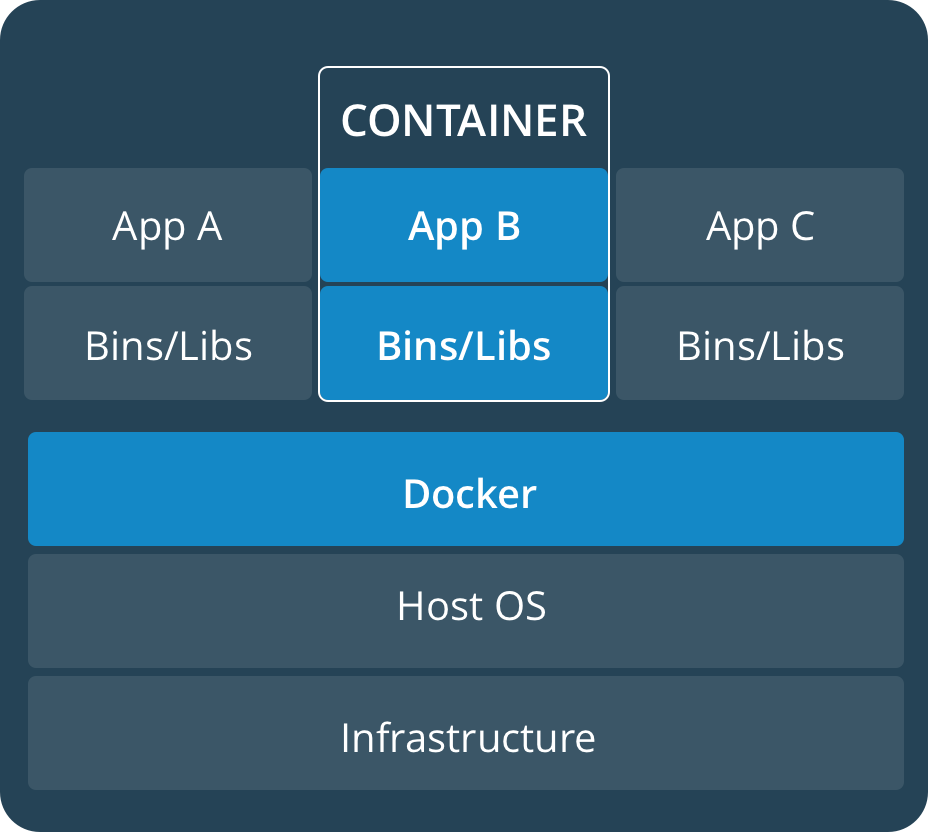
\includegraphics[width=.6\linewidth]{images/docker_container}
    \label{fig:docker_container}
  \end{subfigure}%
  \begin{subfigure}{.5\textwidth}
    \centering
    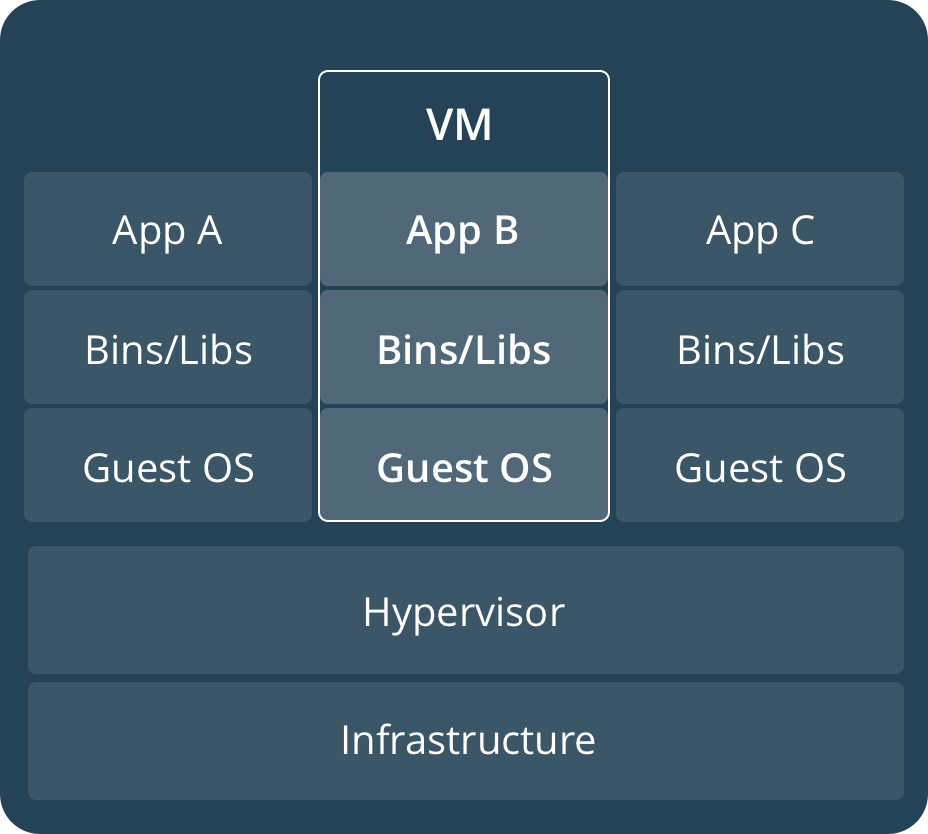
\includegraphics[width=.6\linewidth]{images/docker_vm}
    \label{fig:docker_vm}
  \end{subfigure}
  \caption{Porównanie kontenerów i wirtualnej maszyny.}
\end{figure}

Korzystając z informacji zawartych w dokumentacji Docker'a \cite{docker_what_container}, można wykazać następujące cechy obu rozwiązań:

\begin{itemize}
  \item maszyny wirtualne:
  \begin{itemize}
    \item abstrakcja w warstwie sprzętowej, która zmienia jeden serwer w wiele serwerów,
    \item hipernadzorca (ang. \textit{hypervisor}) pozwala na pracę wielu wirtualnych maszyn na jednej maszynie fizycznej,
    \item każda maszyna wirtualna posiada pełną kopię systemu operacyjnego, aplikacji, niezbędnych bibliotek i ich zależności, przez co zajmuje dużo miejsca na dysku twardym,
    \item maszyny wirtualne zwykle długo się uruchamiają.
  \end{itemize}

  \item kontenery:
  \begin{itemize}
    \item abstrakcja w warstwie aplikacji, która łączy kod z jego zależnościami,
    \item na jednej maszynie może być uruchomionych wiele kontenerów, które wspóldzielą kernel,
    \item każdy z kontenerów jest osobnym procesem w przestrzeni użytkownika,
    \item kontenery zajmują mniej miejsca na dysku i uruchamiają się dużo szybciej, niż maszyny wirtualne.
  \end{itemize}
\end{itemize}

Powyższe zestawienie należy uzupełnić o informacje znajdujące się w prezentacji Łukasza Piątkowskiego \cite{docker_prez}:
\begin{itemize}
  \item maszyny wirtualne:
  \begin{itemize}
    \item wirtualizacja sprzętu - degradacja wydajności,
    \item własny kernel,
    \item pełna maszyna,
  \end{itemize}

  \item kontenery:
  \begin{itemize}
    \item \textit{chroot} z większymi możliwościami,
    \item wspólny kernel,
    \item własne zasoby pamięci, dysku, I/O.
  \end{itemize}
\end{itemize}

Analizując cechy obu rozwiązań można stwierdzić, że kontenery mają sporą przewagę w ważnych kwestiach (wydajność, szybkość uruchamiania, wymagane zasoby) nad maszynami wirtualnymi, dlatego też stają się coraz bardziej popularne.

Ze strony programisty, otrzymuje on nową instancję wybranego systemu, gdzie zainstalowane są jedynie zależności wymagane przez daną aplikację. Prowadzi to do odizolowania środowiska aplikacji, przez co znacząco minimalizowane jest ryzyko wystąpienia konfliktów pomiędzy aplikacjami, aplikację można w bardzo prosty sposób przenieść na inną maszynę i uruchomić ją jedną komendą.

\subsection{CRUD}
CRUD, to cztery podstawowe funkcje w aplikacjach korzystających z pamięci trwałej, które umożliwiają zarządzanie nią \cite{wiki_crud}. Akronim ten powstał od pierwszych liter słów \textbf{C}reate, \textbf{R}ead, \textbf{U}pdate i \textbf{D}elete. Określa on udostępnienie użytkownikowi bądź aplikacji zestaw operacji (stworzenie, odczytanie, aktualizacja oraz usunięcie) na danym obiekcie.


\chapter{Przegląd wybranych rozwiązań}
\section{Ruby on Rails}
Ruby on Rails jest open source'owym frameworkiem webowym. Został stworzony w~głównej mierze przez duńskiego programistę Davida Heinemeiera Hanssona. Pierwsza wersja RoR ukazała się w~lipcu 2004 roku. Fakt ten pokazuje, że jest to już dojrzały framework, z~ugruntowaną pozycją na rynku. Potwierdzeniem tej pozycji jest liczne wsparcie społeczności. Rails'y zostały stworzone przez ponad 4,5 tysiąca osób, istnieje ok. 132 tysiące ogólnodostępnych paczek, które rozszerzają funkcjonalność tego frameworku. Ruby on Rails domyślnie korzysta z~architektury MVC, czyli \emph{Model - View - Controller}.

\subsection{Doktryna Ruby on Rails}
Tworzeniu i~rozwojowi Ruby on Rails towarzyszy kilka podstawowych zasad. Jedne istnieją od początku, inne ewoluowały na przestrzeni lat. Spisane są one w~\emph{The Rails Doctrine} \cite{rails_doctrine}. Na potrzeby pracy zostaną omówione najważniejsze z nich.

\subsubsection{Optimize for programmer happiness}
Pierwsza reguła odnosi się mocno do języka, z~którego wywodzą się Rails'y. Sam fakt umieszczenia nazwy języka Ruby w~nazwie frameworku pokazuje jak ważny jest on dla całego projektu. Motywacją stworzenia języka Ruby była chęć dostarczenia programistom radości z~pisania kodu. w~momencie powstawania Ruby'ego, większość popularnych wtedy języków programowania narzucało sposób pisania bądź stosowało liczne ograniczenia w~sposobie pisania kodu. Ruby stał w~opozycji do tych zasad, dając programistom pełną dowolność w~sposobie tworzenia kodu.

Jako przykład owego ,,uwolnienia'' programisty podawana jest \emph{Zasada Najmniejszego Zaskoczenia} (ang. The Principle of Least Surprise).
\begin{lstlisting}[caption={Wyjście z~interpretera Ruby'ego.},language=Ruby]
$ irb
irb(main):001:0> exit
$ irb
irb(main):001:0> quit
\end{lstlisting}

\begin{lstlisting}[caption={Wyjście z~interpretera Python'a.},language=Python]
$ python
>>> exit
Use exit() or Ctrl-D (i.e. EOF) to exit
\end{lstlisting}
Ruby zaakceptuje oba polecenia opuszczenia interpretera. Python natomiast, pomimo odczytania intencji programisty (wyświetlenie instrukcji), opuści interpreter jedynie po wpisaniu komendy \emph{exit()} lub po użyciu kombinacji klawiszy \emph{Ctrl-D}, co oczywiście nie jest zgodne z~oczekiwaniami programisty.

Wzorując się na zasadach, na których powstawał Ruby, Rails'y również miały umilać życie programistom. Jako przykład jest podawana klasa \emph{Inflector}. Zapisane są w~niej reguły oraz wyjątki od reguł w~języku angielskim, które umożliwiają mapowanie klasy \emph{Comment} na tabelę \emph{Comments}, \emph{Person} na \emph{People} itp. Kolejnym przykładem może być dodatek do Ruby'owej klasy \emph{Array}, który poza dostępnym w~Rubym pierwszym elementem tablicy, umożliwia dostęp do kolejnych czterech elementów tablicy, poprzez wyrażenia \emph{Array\#second,~Array\#third} itd.

Oczywiście nie są to kluczowe cechy frameworku, ale stanowczo zaznaczają ważkość celu, którym jest przede wszystkim sprawianie radości z~tworzenia oprogramowania.

\subsubsection{Convention over Configuration}
Twórcy Ruby on Rails starają się kłaść mocny nacisk na prostotę używania ich narzędzia. Zamiast zrzucać na programistów ciągłe podejmowanie decyzji w~kwestiach mało istotnych, jak na przykład format klucza obcego w~bazie danych, Rails'y narzucają konwencję nazewnictwa. Oczywiście jest możliwość konfiguracji narzuconych przez framework konwencji, lecz jest to raczej rzadko spotykane, a~wręcz niewskazane. Zasada ta, poza zdjęciem odpowiedzialności za część decyzji z~barków programisty, przynosi również inne korzyści.

Dzięki ,,domyślnej'' konwencji, możliwe jest stworzenie głębszej abstrakcji, na której operuje framework. Przykładem może być zastosowanie wcześniej wymienionej klasy \emph{Inflector}. Jeśli możliwe jest zmapowanie klasy \emph{Person} na tabelę \emph{People}, to możliwe jest również zmapowanie relacji \emph{has\_many: people} w~taki sposób, aby wykorzystywana była klasa \textit{Person}. Jest to o~tyle wygodne rozwiązanie, że nawet pomimo posiadania wiedzy na temat tworzenia relacji w~bazie danych oraz sposobu odzwierciedlania ich w~kodzie aplikacji, programista nie musi przejmować się tworzeniem lub konfiguracją tej części aplikacji.

Kolejną zaletą jest znaczące obniżenie progu wejścia dla początkujących programistów. Takim osobom dużo łatwiej jest poznawać framework stopniowo. Począwszy od poziomu, gdzie wszystko automatycznie działa, lecz nie wiadomo dlaczego, aż do momentu gdzie nadal wszystko automatycznie działa, ale bardzo dobrze wiadomo dlaczego. Znaczna część mechanizmów stosowanych we frameworkach webowych \emph{de facto} nie wymaga niestandardowej konfiguracji, nawet jeśli programista posiada szeroką wiedzę w~danej dziedzinie. Przekładanie konfiguracji ponad konwencję wymaga od programisty sporego wysiłku, aby rozpocząć pracę z~frameworkiem, co w przypadku poznawania nowych technologii stanowczo nie jest zachęcające.

Zasada ta bywa jednak zgubna. Jest tak z~powodu błędnego przekonania, że skoro od samego początku wszystkie elementy aplikacji można wygenerować, i~od samego początku wszystko działa, to programista nie musi mieć wiedzy na temat tego, co robi. W~przypadku bardzo podstawowych zastosowań wiedza programisty rzeczywiście nie musi być szeroka, natomiast bardzo problematyczne jest w~takim przypadku wykonanie części aplikacji, która jest niestandardowa bądź niemożliwa do wygenerowania.

\subsubsection{The menu is omakase}
Rzadko kiedy framework jest monolitem, który nie składa się z~modułów. Częściej framework jest zbiorem mniejszych frameworków lub bibliotek, które współpracują ze sobą. Bardzo często wybór owych narzędzi leży w~pełni po stronie programisty. Jako analogię takiego wyboru, w \emph{The Ruby on Rails Doctrine} podawany jest problem wyboru dania z~menu w~restauracji, którą odwiedzamy po raz pierwszy. Jeśli zdamy się na wybór szefa kuchni, możemy założyć że jedzenie będzie dobre, nie wiedząc jeszcze co ,,dobre'' będzie oznaczać \cite{rails_doctrine}.

Ruby on Rails rozwiązuje ten problem poprzez dostarczenie zestawu narzędzi, z~których programista może korzystać. Zasada działania jest tutaj bardzo zbliżona do reguły \emph{Convention over Configuration}, lecz operuje na wyższym poziomie abstrakcji. Programista dostaje zestaw domyślnych narzędzi, z~którego może od samego początku korzystać, bez potrzeby podejmowania decyzji odnośnie wyboru frameworków i~bibliotek. Ma on natomiast możliwość zamiany domyślnie wybranych narzędzi na inne, jeśli widzi taką potrzebę.

Zasada ta niesie za sobą korzyści w~sferze rozwoju frameworku. Jest tak, ponieważ programiści, używając tych samych narzędzi, są w~stanie bardziej dopracować owe narzędzia. Częstym problemem jest nie fakt jak działa dany framework bądź biblioteka w~izolacji, lecz jak działa razem z~innymi modułami. Jeśli wielu programistów napotyka te same błędy w~integracji poszczególnych składowych frameworku, to dużo łatwiej jest twórcom takie błędy poprawić bądź usprawnić połączenie tych modułów.

\subsubsection{No one paradigm}
Twórcy frameworka Ruby on Rails są przekonani, że nie istnieje jedno idealne rozwiązanie. Często do jednego celu można dojść różnymi drogami. Z~tego też powodu, pomimo wyboru architektury MVC, Railsy są bardzo elastyczne jeśli chodzi o~dostosowanie się do innych modeli projektowych. Domyślnie RoR nie posiada wbudowanych \textit{Serwisów} bądź \textit{Prezenterów}, lecz framework jest zbudowany w~taki sposób, aby użycie większości wzorców projektowych było bezproblemowe.

Przystosowanie frameworku do korzystania z~różnych wzorców projektowych poniekąd wymusza na programistach znajomość większej ilości owych wzorców. Jako, że Ruby jest bardzo elastycznym językiem jeśli chodzi o~paradygmaty programowania, ponieważ możliwe jest pisanie funkcyjne, Railsy również wspierają owe podejście. Od programisty zależy, czy z~takiej możliwości skorzysta. Wprowadzenie takiej uniwersalności niestety niesie za sobą spory nakład pracy ze strony twórców.

\subsection{Pozostałe cechy}
Poza cechami wymienionymi w \textit{The Ruby on Rails Doctrine}, Ruby on Rails kładzie mocny nacisk na inne aspekty. Są to m.in. kwestie takie, jak przestrzeganie reguły \textit{DRY} (ang. \textit{Don't Repeat Yourself}) bądź też wsparcie dla dodatkowych bibliotek rozszerzających funkcjonalność frameworku.

\subsubsection{Don't Repeat Yourself}
Reguła \textit{DRY} mówi o tym, aby, jak sama nazwa wskazuje, nie powtarzać kodu. Każde powtórzenie logiki biznesowej może być rozwiązane poprzez dodanie warstwy abstrakcji. Natomiast duplikację procesów można rozwiązać poprzez ich automatyzację \cite{dry}. Poprzez stosowanie tej reguły, kod aplikacji jest wyraźnie mniejszy, ale przede wszystkim jest on bardziej odporny na błędy i łatwiejszy w utrzymaniu. Jeśli w~powtarzającym się fragmencie kodu zostanie popełniony błąd, dzięki zastosowaniu reguły DRY, zmianę trzeba wprowadzić tylko w~jednym miejscu, a~nie w~każdym wystąpieniu powtarzającej się funkcji.

Ruby on Rails wspiera używanie tej reguły poprzez wbudowane w framework elementy, takie jak \textit{Helpery}, \textit{Concerny} lub \textit{Partiale}. Umożliwiają one wspóldzielenie kodu i używanie ich w każdej z warstw aplikacji.

\subsubsection{Biblioteki}
Biblioteki tworzone przez społeczność nie są bezpośrednio elementem frameworku, ale samego języka Ruby. Ich nazwa to \textit{gem'y}. Rails'y natomiast mają domyślnie dołączony menedżer bibliotek/pakietów - \textit{bundler}.

\begin{figure}[h]
  \centering
  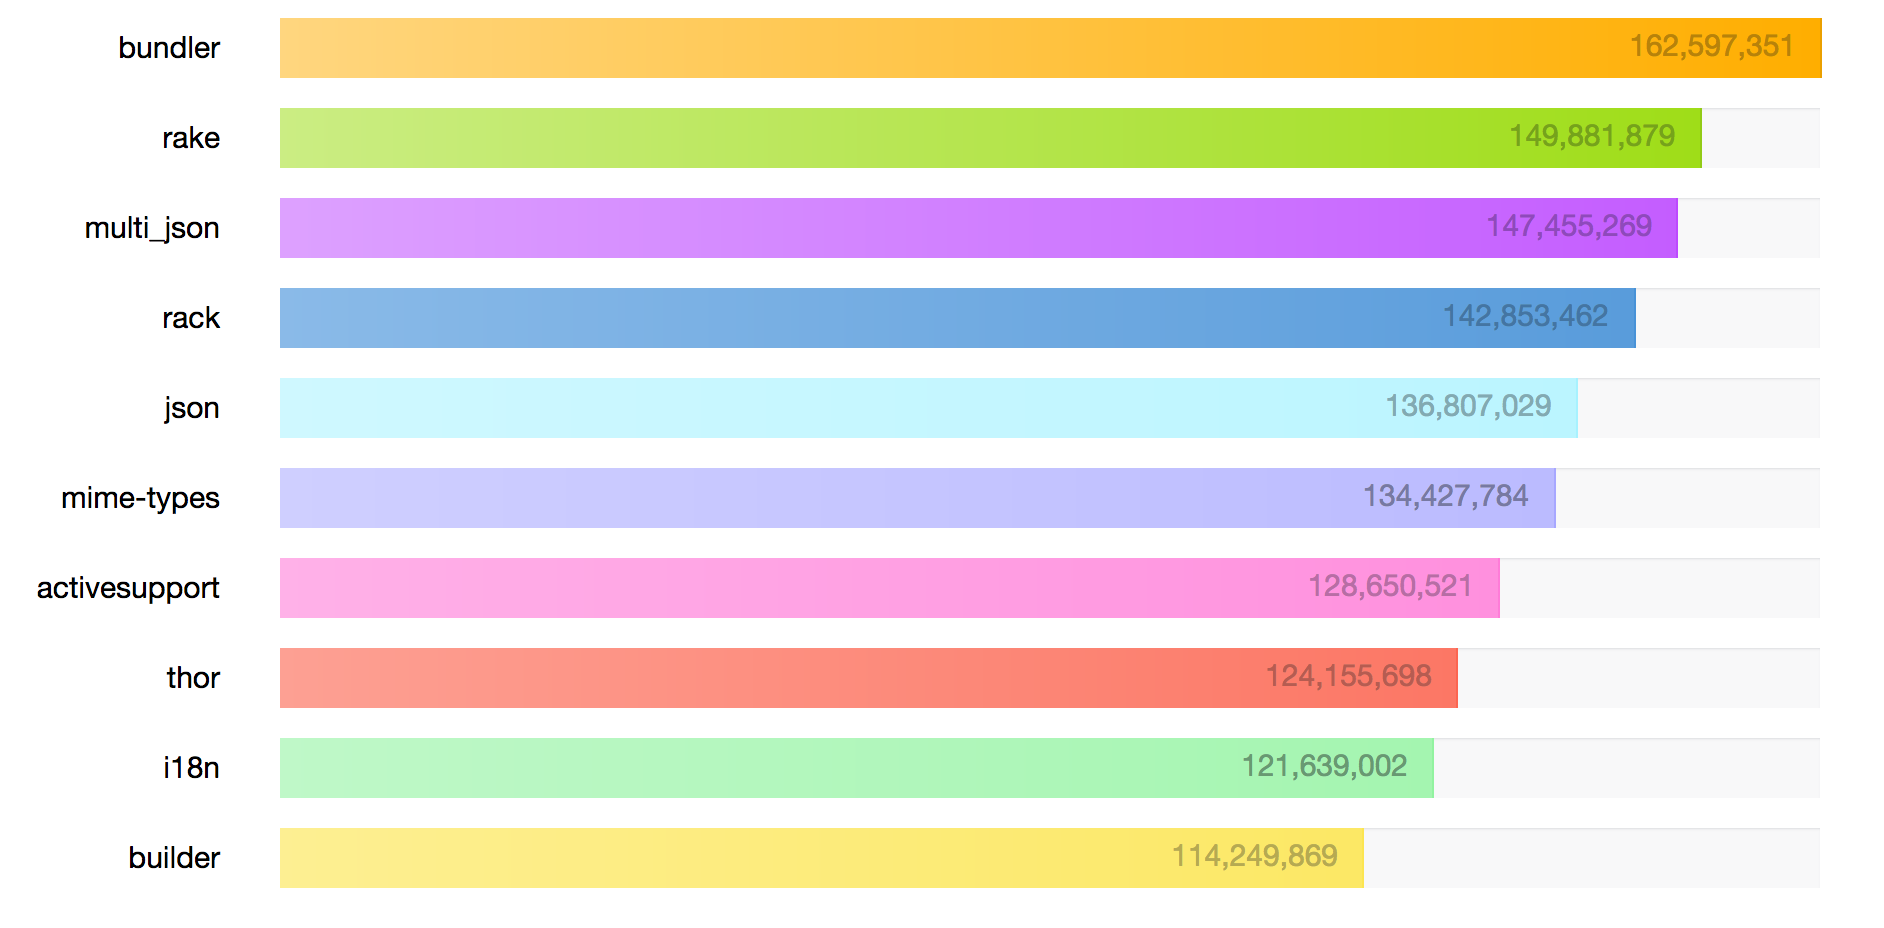
\includegraphics[width=\linewidth]{images/bundler_stats}
  \caption{Statystyki pobrań menedżera pakietów bundler.\\Źródło: \url{https://rubygems.org/stats}}
  \label{fig:bundler_stats}
\end{figure}

Jak widać, \textit{bundler} jest najczęściej pobieranym \textit{gem'em} spośród wszystkich, z ilością pobrań przekraczającą 162,5 miliona. Ogromny wpływ na taki wynik mają oczywiście Rails'y. Strona \url{https://rubygems.org/}, która jest źródłem większości bibliotek, w statystykach podaje, że dostępnych jest ponad 131,600 paczek. Pokazuje to jak ważną częścią dla twórców Ruby on Rails i całej społeczności jest możliwość tworzenia rozszerzeń oraz ich dostępność.

\section{Phoenix} % https://media.pragprog.com/titles/phoenix/intro.pdf   http://www.phoenixframework.org/docs/resources

\textit{Phoenix} jest open source'owym frameworkiem webowym napisanym w języku \textit{Elixir}. Inicjatorem tego projektu jest amerykanin Chris McCord. Pierwsza wersja \textit{Phoenix'a} została wydana 28 sierpnia 2015 roku, a więc jest to bardzo młody framework. Pomimo swojego młodego wieku, framework ten zyskał sporą popularność i zainteresowanie społeczności. Jest to spowodowane ideą frameworku, który nie stara się być na siłę inny od istniejących rozwiązań, a zamiast tego stara się wykorzystywać ich najlepsze elementy. Jako przykładowe frameworki, z których czerpie \textit{Phoenix}, wymieniane są \textit{Ruby on Rails} oraz \textit{Django} \cite{phoenix_docs}.

Tak, jak większość frameworków webowych, \textit{Phoenix} implementuje wzorzec \textit{Model-View-Controller}.

\subsection{Podstawowe założenia}
Idea działania \textit{Phoenix'a} opiera się na kilku podstawowych założeniach:
\begin{itemize}
  \item szybkość działania,
  \item współbieżność,
  \item wygoda użytkowania,
  \item niezawodność.
\end{itemize}

\subsubsection{Szybkość działania}
Położenie nacisku na szybkość działania aplikacji stworzonej przy pomocy frameworka jest czymś naturalnym. Zwykle jednak szybkość działania osiągana jest kosztem innych aspektów tworzenia aplikacji, jak na przykład szybkością powstawania oprogramowania. Aby osiągnąć zadowalającą szybkość działania, twórcy \textit{Phoenix'a} zdecydowali się stworzyć framework przy pomocy języka \textit{Elixir}. Wpływ tego języka na framework opisany jest szerzej w sekcji \ref{phoenix:elixir}.

Poza samym językiem programowania, na szybkość działania aplikacji wpływ mają następujące rozwiązania:
\begin{itemize}
  \item router kompilowany jest do bardzo szybkiego w działaniu \textit{pattern matching'u}, czyli dopasowaniu do wzorca. Dzięki temu optymalizacja wydajności wykonywana jest jeszcze zanim zapytanie opuści router,
  \item template'y są prekompilowane, \textit{Phoenix} nie musi kopiować łańcuchów tekstowych dla każdego wyświetlanego template'u, przez co możliwe jest bardzo wydajne cache'owanie.
\end{itemize}

\subsubsection{Współbieżność}
Wraz z rozwojem możliwości sprzętowych, a dokładniej z rosnącą liczbą rdzeni procesorów, możliwe jest coraz większe wykorzystanie współbieżności w aplikacjach internetowych. Większość frameworków opartych jest na językach obiektowych, co niestety generuje problemy w kwestii współbieżności. Jest tak, ponieważ aby skorzystać z mechanizmu współbieżności, programista musi taką funkcjonalność zaimplementować, oczywiście przy pomocy dostępnych w języku narzędzi. Niestety, współbieżność nie jest prostym zagadnieniem, posiada wiele pułapek, przez co programiści, jeśli nie muszą, zwykle z niej nie korzystają.

Współbieżność, podobnie jak szybkość działania, jest cechą, która osiągnięta została poprzez wybór odpowiedniego języka programowania. \textit{Elixir}, jako język funkcyjny stworzony do tworzenia bardzo wielu procesów, w pełni spełnia wymogi stawiane przez twórców \textit{Phoenix'a}. Nie tylko posiada on bardzo wydajne mechanizmy zapewniające współbieżność, ale przede wszystkim bardzo ułatwia korzystanie z owej współbieżności. I owe ułatwienie pracy programisty jest ważnym czynnikiem popularności \textit{Phoenix'a}. Przykład łatwości korzystania z mechanizmu współbieżności znajduje się na listingu \ref{lst:phoenix_concurrency}, który pochodzi z pozycji literaturowej \cite{phoenix_doctrine}.

\begin{lstlisting}[label={lst:phoenix_concurrency}, caption=Współbieżność w Phoenix'ie]
company_task = Task.async(fn -> find_company(cid) end)
user_task = Task.async(fn -> find_user(uid) end)
cart_task = Task.async(fn -> find_cart(cart_id) end)

company = Task.await(company_task)
user = Task.await(user_task)
cart = Task.await(cart_task)
\end{lstlisting}

Dzięki tak prostym interfejsom, wykonanie kodu z listingu \ref{lst:phoenix_concurrency} zajmie tyle, ile najdłuższe zapytanie do bazy danych, a nie łączny czas zapytań. Dzięki temu dużo lepiej wykorzystywana jest baza danych, co przekłada się na szybkość działania całej aplikacji.

\subsubsection{Wygoda użytkowania}
Wygoda użytkowania jest wypadkową wielu czynników. Z jednej strony jest to wybrany język programowania, który udostępnia programiście w przystępny sposób wiele zaawansowanych mechanizmów, ma ,,przyjazną'' składnię i jest dość prosty w nauce. Z drugiej strony \textit{Phoenix} w swoich założeniach chce się wzorować na innych frameworkach wykorzystując ich najlepsze elementy. Tak więc programista korzysta z rozwiązań, które mogą być mu znane z innych technologii, jak na przykład \textit{Django} lub \textit{Laravel}, co dodatkowo przyspiesza powstawanie aplikacji webowych.

\subsubsection{Niezawodność}
Niezawodność jest podstawą każdej aplikacji, nie tylko internetowej. Nawet najładniejszy, współbieżny i responsywny kod jest bezwartościowy, jeśli nie jest niezawodny. Aplikacje pisane w \textit{Erlang'u} zawsze były bardziej niezawodne od innych, głównie poprzez strukturę linkowania procesów oraz komunikację pomiędzy procesami, co pozwala na efektywną pracę \textit{supervisor'a} \cite{phoenix_doctrine}.

Po raz kolejny jedno z głównych założeń frameworka jest głęboko zakorzenione w przeznaczeniu języka programowania. Wysoka niezawodność jest oczywiście celem praktycznie wszystkich aplikacji, ponieważ błędy aplikacji są bardzo kosztowne dla ich właścicieli.

Dla programistów niezawodność fundamentów, na których budują funkcjonalność aplikacji, jest nieoceniona. Dużo łatwiej tworzy się aplikację mając pewność, że abstrakcje nałożone przez framework są wydajne i niezawodne, przez co można skupić się na tworzeniu funkcjonalności.

\subsection{Elementy składowe}
\textit{Phoenix} jest nadrzędną warstwą w wielowarstwowym systemie zaprojektowanym, aby być modularnym i elastycznym. Pozostałe warstwy zawierają narzędzia takie jak \textit{Plug} (odpowiedzialny za modularność), \textit{Ecto} (odpowiedzialny za interakcję z bazą danych), \textit{Cowboy} (serwer HTTP Erlanga) \cite{phoenix_docs}.

Efektem połączenia wszystkich warstw są następujące elementy:
\begin{itemize}
  \item \textbf{endpoint}, który jako pierwszy zajmuje się zapytaniami, odpowiednio je obsługuje i przekazuje do routera,
  \item \textbf{router} - parsuje przychodzące zapytania i przekierowuje je do odpowiednich kontrolerów i akcji,
  \item \textbf{kontroler} - dostarcza on akcje, które obsługują zapytanie (przetwarzanie danych, przekazanie ich do widoków, generowanie HTML przekazywanych do przeglądarki),
  \item \textbf{szablony} - w połączeniu z danymi oraz po pewnym przetworzeniu generują widoki,
  \item \textbf{widoki}, które są warstwą prezentacji, czyli wizualnym efektem działania aplikacji,
  \item \textbf{kanały} - zarządzają websocketami, które umożliwają komunikację w czasie rzeczywisttym pomiędzy serwerem, a klientem.
\end{itemize}

\subsection{Język programowania - Elixir} % https://elixir-lang.org/
\label{phoenix:elixir}
Podobnie, jak w przypadku \textit{Ruby on Rails}, duży wpływ na jakość użytkowania \textit{Phoenix'a} ma język programowania, w którym jest on stworzony. \textit{Elixir} jest kompilowanym językiem funkcyjnym, który uruchamiany jest na maszynie wirtualnej \textit{Erlanga}. Dodatkowo, jak piszą jego twórcy, jest językiem programowania zaprojektowanym do tworzenia skalowalnych i łatwych w utrzymaniu aplikacji \cite{elixir}.

Wybór tego języka programowania umożliwia zrealizowanie jednych z podstawowych zadań \textit{Phoenix'a} - zapewnienie wysokiej wydajności oraz niezawodności.

Dodatkowo twórcy zwracają uwagę na przyjazną składnię, co stanowczo ma wpływ na popularność frameworka. Jest tak, ponieważ programiści zwykle wolą czerpać przyjemność z używania ,,ładnego'' języka, niż uczyć się i używać mało przyjaznego języka programowania. \textit{Elixir}, jako pierwszy funkcyjny język programowania, wspiera makra z rodziny języków \textit{Lisp}, lecz robi to stosując bardziej naturalną składnię \cite{phoenix_doctrine}.

\subsection{Pozostałe cechy}
\subsubsection{Biblioteki}
Idea centralnego repozytorium paczek jest bardzo popularna wśród większości języków programowania. Ułatwia ono pracę w aplikacją, dodawanie nowych zależności nie jest problematyczne, a błędy dotyczące niezgodności wersji zależności są wyeliminowane. Dla języka \textit{Elixir} domyślnym menadżerem paczek jest \textit{Hex}.

\begin{figure}[h]
  \centering
  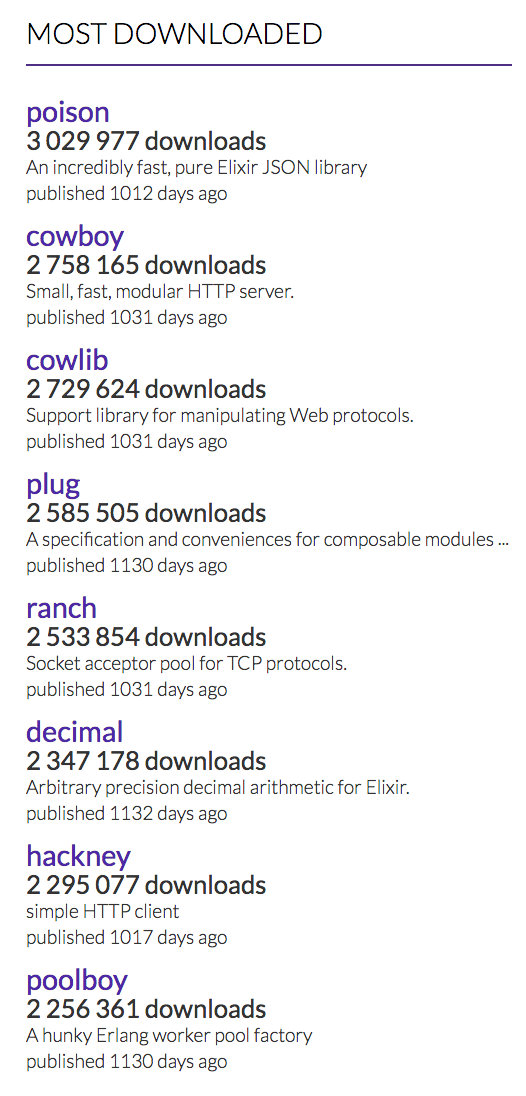
\includegraphics[width=.4\linewidth]{images/hex_stats}
  \caption{Statystyki pobrań menedżera pakietów Hex.\\Źródło: \url{https://hex.pm/}}
  \label{fig:hex_stats}
\end{figure}

W momencie powstawania niniejszej pracy, dostępnych jest ok 4,5 tysiąca bibliotek w oficjalnym repozytorium  \textit{Hex}. W porównaniu do innych, będących na rynku dłużej języków i frameworków, jest to niewielka liczba. Biorąc natomiast pod uwagę rosnącą popularność \textit{Phoenix'a}, można założyć iż ta liczba będzie rosnąć. Obecnie istniejące paczki są niekiedy odpowiednikami istniejących już paczek napisanych w innych językach. Niestety, bardzo często paczki te, z racji na krótki okres istnienia, są mocno niedopracowane.

\section{Express}
\textit{Express} jest minimalistycznym i bardzo elastycznym frameworkiem webowym. Framework ten powstał poprzez dostarczenie wrapperów dla API udostępnianego przez platformę \textit{Node.js}. \textit{Express}, ze względu na swoją budowę, można traktować jako podstawę do budowy innych frameworków. Framework ten jest dostępny jako wolne oprogramowanie pod licencją MIT i komercyjnie wspierany jest przez firmę \textit{StrongLoop}. \textit{Express} nie jest frameworkiem typu \textit{full-stack}, jest on nastawiony na możliwość dowolnej konfiguracji zależności niezbędnych w projekcie.

\subsection{Podstawowe założenia}
% http://noeticforce.com/best-nodejs-frameworks-for-web-and-app-development
% Sinatra inspired!!!
Pierwotną ideą powstania \textit{Express'a} była chęć stworzenia frameworka podobnego do istniejącego w języku programowania \textit{Ruby} frameworka \textit{Sinatra}. Z tego względu oba te frameworki współdzielą podejście do rozwiązywania problemów oraz struktury kodu.

\subsubsection{Configuration over convention}
Głównym założeniem frameworka \textit{Express} jest dostarczenie programistom pełnej elastyczności i możliwości wyboru poszczególnych składowych aplikacji. W skład frameworku nie wchodzą więc biblioteki odpowiedzialne m.in. za:
\begin{itemize}
  \item komunikację z bazą danych,
  \item autentykację użytkowników,
  \item silnik szablonów.
\end{itemize}

Zastosowanie podejścia \textit{configuration over convention} może być problematyczne w przypadku rozpoczynania swojej przygody z \textit{Express'em}. W sytuacji, kiedy framework nie dostarcza wbudowanych mechanizmów, jak np. wcześniej wymieniony adapter do bazy danych, programista nie znający dostępnych bibliotek może mieć duże problemy z wyborem odpowiedniego mechanizmu.

\subsubsection{Organizacja struktury aplikacji}
Ze względu na podejście \textit{convention over configuration}, \textit{Express} nie narzuca programistom konkretnej struktury aplikacji. W żaden sposób nie jest wyróżnione podejście, które najczęściej można spotkać w aplikacjach webowych, czyli \textit{Model-View-Controller}. Programista może wybrać dowolny wzorzec projektowy, bądź też nie zastosować żadnego, jeśli taka jest jego wola.

\subsection{Podstawa dla innych frameworków}
% typy zbudowanych frameworków + nazwy
\textit{Express} bez żadnych dodatkowych bibliotek, czyli od razu po instalacji, nie dostarcza wielu, niekiedy ważnych, funkcjonalności. Programiści korzystający z tego frameworka potrzebowali jednak tych samych narzędzi w przypadku tworzenia aplikacji tego samego typu. W momencie, kiedy za każdym razem musieli dołączać do projektu i konfigurować te same biblioteki, zaczęły powstawać bardziej ,,kompletne'' frameworki, które bazowały na \textit{Expressie}. W ten sposób powstały następujące frameworki:
\begin{itemize}
  \item LoopBack - stworzony do budowy REST API,
  \item ItemsAPI - framework łączący funkcjonalność \textit{Elastichsearch'a} i \textit{Express'a},
  \item KeystoneJS - \textit{Content Management System},
  \item MEAN - framework typu full-stack,
  \item Feathers - stworzony do budowy REST API,
  \item Sails.js - framework MVC typu full-stack,
  \item Hydra-Express - framework stworzony do architektury mikroserwisów.
\end{itemize}

\subsection{Biblioteki}
Większość języków programowania posiada swój menedżer paczek, nie inaczej jest w przypadku języka \textit{JavaScript}. W tym środowisku największą popularność zyskał \textit{npm}. Jako, że \textit{npm} jest menedżerem paczek języka, a nie frameworka, można tam oczywiście znaleźć paczki niekompatybilne z \textit{Expressem}, lecz jest to cecha wszystkich menedżerów stworzonych dla konkretnego języka programowania.

Na oficjalnej stronie \textit{npm} \cite{npm_site} przeczytać można, że dostępnych jest ponad 470 tysięcy paczek. Z repozytorium \textit{npm} tygodniowo pobieranych jest 2 365 813 490 paczek.


\chapter{Analiza porównawcza}
Naturalnym jest, że frameworki webowe różnią się od siebie pod wieloma względami. Różnice można zauważać od samego początku, czyli idei powstania, poprzez podejście do programisty, na sposobie działania i wydajności kończac. Zwykle przyczyną różnorodności jest sama filozofia frameworka, dążenie do doskonałości. Nie jest możliwe osiągnięcie optymalnych wartości w każdej z dziedzin, które frameworki obejmują, przez co twórcy muszą iść na większe bądź mniejsze kompromisy. Niekiedy owe różnice nie pojawiają się z przymusu, ale z przyjęcia konkretnych założeń.

Są jednak sytuacje, kiedy frameworki są do siebie bardzo podobne. Zwykle są to sytuacje, kiedy framework z jednego języka programowania przenoszony jest do innego języka. Tak było w przypadku opisywanego \textit{Express'a}, który powstał jako odzwierciedlenie frameworka \textit{Sinatra}. Innym przypadkiem występowania podobieństw jest chęć wykorzystania jakiegoś fragmentu frameworka, który uznawany jest za standard i bez którego programista musi posiadać większą wiedzę aby odpowiednio wykorzystywać framework.\\

W kolejnych podrozdziałach zostaną przedstawione porównania wybranych frameworków na zasadzie \textit{,,każdy z każdym''}. Poza podobieństwami i różnicami w budowie oraz idei działania, zamieszczona została subiektywna opinia autora na temat sytuacji, w których jeden framework ma przewagę nad drugim.

\section{Ruby on Rails vs Phoenix}
Jako pierwsze analizie porównawczej zostaną poddane najstarszy i najmłodszy framework spośród opisywanych, czyli \textit{Ruby on Rails} oraz \textit{Phoenix}. Owa różnica ,,wieku'' mocno rzutuje na całokształ tych frameworków.  Pierwszy ma już stabilną, wręcz nienaruszalną, pozyję na rynku, bardzo dużą społeczność oraz niezliczoną ilość materiałów dostępnych w Internecie.
Drugi natomiast, co oczywiście jest efektem wielu składowych, ma spory potencjał. Oczywiście nie jest to pierwszy, ani jedyny, framework, który owy potencjał posiada. Jednakże w przypadku \textit{Phoenix'a} jest duża szansa, iż będzie on wykorzystany. Przyczynić się do tego może środowisko programistów \textit{Ruby on Rails}, ponieważ już teraz duża ilość programistów albo mocno się \textit{Phoenixem} interesuje, albo zdecydowało się zmienić technologię na \textit{Elixir'a} i \textit{Phoenix'a}.

% !!filozofia działania
% idea powstania
% !!architektura, elementy składowe
% !!wygoda użytkowania
% szybkość powstawania aplikacji
% !!dostępność najczęściej wykorzystywanych bibliotek (system użytkowników, zapisywanie plików w chmurze, przetwarzanie w tle)
% testowanie aplikacji

\subsection{Filozofia działania}
\textit{Ruby on Rails} oraz \textit{Phoenix} posiadają elementy wspólne jeśli chodzi o sposób działania. Jest to spowodowane faktem, iż z założenia \textit{Phoenix} miał wykorzystywać najlepsze elementy z innych frameworków.

Jeśli chodzi o filozofię działania, oba frameworki są zgodne w kwestii chęci ułatwienia pracy programistom. Zarówno \textit{Ruby on Rails}, jak i \textit{Phoenix}, mocno uwypuklają przyjemność korzystania z języków programowania, na których są oparte. Twórcy \textit{Ruby on Rails} zapoczątkowali trend stawiania na przyjemność użytkowania w świecie frameworków webowych, natomiast twórcy \textit{Phoenix} bardzo dobrze to zaimplementowali w swoim frameworku. Z tego też powodu spora część programistów \textit{Ruby on Rails} interesuje się rozwojem \textit{Phoenix'a}.\\

Podstawową różnicą w filozofii działania jest kwestia szybkości działania. Twórca \textit{Ruby on Rails} nie poświęcił ani jednego punktu w \emph{,,The Ruby on Rails Doctrine''} \cite{rails_doctrine}. Można z tego faktu wyciągnąć wniosek, że szybkość działania \textbf{nie jest} kluczowa dla tego frameworka. I powszechna opinia na temat \textit{Rails'ów} to potwierdzi. Nie zmienia to jednak faktu, że wiele bardzo dużych portali opartych jest na \textit{Ruby on Rails}. Przykładami mogą być \textit{GitHub}, \textit{Groupon}, \textit{AirBnB} czy \textit{Kickstarter}. Framework ten jest natomiast idealnym narzędziem do szybkiego tworzenia aplikacji. \textit{Ruby on Rails} na pewno zyskało wielu użytkowników ze względu na szybkość prototypowania, co jest bardzo istotne w dobie \textit{start-up'ów}.

Dla odmiany, \textit{Phoenix} szczyci się swoją wysoką wydajnością. Jest to jeden z filarów tego frameworka. Co ciekawe, pomimo postawienia na szybkość działania, nie ucierpiała na tym szybkość prototypowania. Powodów takiego stanu rzeczy po raz kolejny można doszukiwać się w języku programowania, na którym oparty jest \textit{Phoenix}. Tworzy to sporą przewagę nad \textit{Ruby on Rails} w przypadkach, gdzie poza szybkością powstania aplikacji równie ważna jest jej wydajność.

\subsection{Architektura aplikacji, elementy składowe}
Zarówno \textit{Ruby on Rails}, jak i \textit{Phoenix} są frameworkami typu full-stack. Oznacza to, że dostarczane są z mechanizmami odpowiedzialnymi za:
\begin{itemize}
  \item serwer http - przy pomocy którego można uruchomić aplikację w środowisku developerskim,
  \item generowanie struktury projektu (architektura MVC),
  \item połączenie z bazą danych - adaptery do różnych typów baz danych, ORM,
  \item router aplikacji - odpowiedzialny za przekierowywanie zapytań do odpowiednich akcji kontrolerów,
  \item podstawowe mechanizmy bezpieczeństwa (mechanizm sesji, bezpieczne ciasteczka),
  \item silniki szablonów - Slim, HAML,
  \item wysyłanie wiadomości e-mail z aplikacji - należy jedynie skonfigurować serwer SMTP z którego ma korzystać aplikacja.
\end{itemize}

Wykorzystywana w obu frameworkach architektura została pokazana na rysunku \ref{fig:rails_architecture}.
\newpage
% http://www.sentex.net/~pkomisar/Ruby/Rails2.png (?)
\begin{figure}[h]
  \centering
  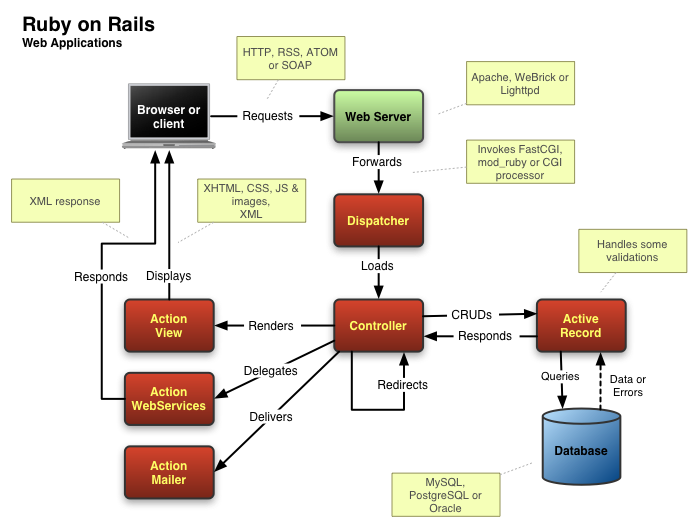
\includegraphics[width=\linewidth]{images/rails_architecture}
  \caption{Architektura Ruby on Rails.}
  \label{fig:rails_architecture}
\end{figure}

\subsection{Wygoda użytkowania, szybkość powstawania aplikacji}
W kwestii wygody użytkowania oba frameworki są na podobnym poziomie. Zarówno \textit{Ruby on Rails} jak i \textit{Phoenix} są stworzone w taki sposób, aby ułatwić prototypowanie aplikacji. Dzięki temu odczucia z użytkowania obu są bardzo przyjemne. Aplikacje można tworzyć relatywnie szybko, frameworki posiadają praktycznie wszystkie niezbędne mechanizmy, które wykorzystywane są w większości aplikacji webowych.

Przykładowe mechanizmy, które były brane pod uwagę:
\begin{itemize}
  \item przetwarzanie danych w tle - w przypadku \textit{Ruby on Rails} jest to \textit{Sidekiq}, jego odpowiednikiem w \textit{Phoenix'ie} jest \textit{Akira},
  \item autentykacja/autoryzacja użytkowników, zarządzanie sesją - \textit{Devise} dla \textit{RoR} oraz \textit{Addict} dla \textit{Phoenix'a},
  \item wsparcie dla dołączania skryptów JavaScript w warstwie prezentacji,
  \item wsparcie dla różnych preprocesorów styli (Sass, Less)
\end{itemize}

Istnieje jednak pewna różnica, która może mieć wpływ na wygodę programisty, a jest nim rodzaj języka programowania. Dużo bardziej popularne jest podejście obiektowe, na którym oparty jest \textit{Ruby}. \textit{Elixir} natomiast jest językiem funkcyjnym. Paradygmat funkcyjny różni się znacznie od obiektowego, przez co w przypadku braku znajomości tego paradygmatu, używanie \textit{Phoenix'a} może być dużo trudniejsze. Zasada ta działa oczywiście w dwie strony i jeśli ktoś nie zna podejścia obiektowego, korzystanie z \textit{Ruby on Rails} również może być utrudnione.

\subsection{Podsumowanie}
Oba frameworki są do siebie podobne w kwestii używania. Bardzo ciekawe oraz pomocne są materiały, które wyjaśniają dlaczego dany framework powstał oraz jak powinien być używany, aby w pełni wykorzystać jego potencjał. Przewagą \textit{Ruby on Rails} jest na pewno dojrzałość oraz ogromna społeczność. W kwestii, oczywiście subiektywnej, przyjemności z korzystania, oba frameworki są na podobnym poziomie. \textit{Phoenix} zyskuje przewagę w kwestii wydajności. Moim zdaniem w tym frameworku drzemie niesamowity potencjał i mam nadzieję, że na stałe wpisze się w zbiór najbardziej popularnych frameworków webowych.

\section{Ruby on Rails vs Express}
Zestawienie \textit{Ruby on Rails} oraz \textit{Express'a} jest zestawieniem najstarszych frameworków spośród narzędzi wybranych do analizy. Pierwszy powstał w 2004 roku, drugi natomiast swój początek miał w 2010r. Ze względu na swój wiek oba frameworki mają ugruntowaną pozycję na rynku oraz rzesze użytkowników.

\subsection{Filozofia działania}
W przypadku zestawienia \textit{Ruby on Rails} oraz \textit{Express'a} filozofia działania oraz sama idea powstania są kluczowymi aspektami. Wynika to z faktu, iż \textit{Express} powstał z chęci przeniesienia frameworka \textit{Sinatra} z środowiska programistów Rubiego do środowiska \textit{Node.js}. Framework \textit{Sinatra} powstał natomiast jako kontra do rozbudowanego \textit{Ruby on Rails}. Z tego też powodu \textit{Ruby on Rails} oraz \textit{Express.js} są swoimi przeciwnościami.

Z jednej strony mamy framework typu full-stack i podejście \textit{Convention over Configuration}. Z drugiej - minimalistyczny framework, do którego możemy (ale nie musimy) dołączyć szereg bibliotek, żeby w kwestii funkcjonalności zrównać się z \textit{Ruby on Rails} oraz oczywiście podejście \textit{Configuration over Convention}. Przejście z jednego świata do drugiego bywa dość nieprzyjemne, wymaga dużej czujności programisty oraz większych nakładów pracy. Dlatego też środowiska programistów \textit{Ruby on Rails} oraz \textit{Express'a} rzadko kiedy się przenikają.

Ze względu na ideę powstania każdego z nich, trudno wskazać elementy łączące \textit{Ruby on Rails} oraz \textit{Express'a}. Oba służą do tworzenia aplikacji internetowych, robią to jednak w różny sposób.

\subsection{Architektura aplikacji, elementy składowe}
\label{rails_express:architektura}
Różnice w kwestii architektury aplikacji oraz bibliotek, które się składają na framework, są w przypadku \textit{Ruby on Rails} oraz \textit{Express'a} bardzo łatwe do zauważenia. Wynika to ze złożoności samych frameworków, a więc podejścia typu \textit{full-stack} w przypadku \textit{Ruby on Rails} oraz minimalizmu \textit{Express'a}. Pierwszy posiada praktycznie wszystko, co jest wymagane do stworzenia podstawowej aplikacji internetowej. W przypadku \textit{Express'a} niestety wymagany jest dodatkowy wysiłek programisty w celu stworzenia aplikacji. Podstawowym problemem jest brak dołączonych adapterów umożliwiających połączenie z bazą danych. Framework ten nie posiada również mechanizmu umożliwiające mapowanie obiektowo-relacyjne (ang. \textit{ORM} - Object-Relational Mapping).

Jako, że \textit{Express} nie posiada wbudowanego generatora projektu, projekt nie posiada określonej struktury. Z jednej strony daje to swobodę działania programiście, czego niekiedy brakuje w \textit{Ruby on Rails}. Niewątpliwie możliwość wykorzystania innej architektury aplikacji niż MVC jest mile widzianą cechą. Z drugiej zaś strony może być problematyczne w sytuacji, kiedy każdy projekt ma swoją ,,autorską'' strukturę i nie przestrzega żadnego schematu.

\subsection{Wygoda użytkowania, szybkość powstawania aplikacji}
Porównianie wygody użytkowania oraz szybkości powstawania aplikacji w przypadku \textit{Ruby on Rails} oraz \textit{Express'a} w dużym stopniu odnosi się do sekcji \ref{rails_express:architektura}. Struktura aplikacji oraz biblioteki dołączone do frameworka są kluczowe dla programistów, szczególnie początkujących. W połączeniu z brakiem domyślnych mechanizmów mapowania obiektowo-relacyjnego, można odnieść wrażenie, iż \textit{Express} nie jest najlepszym frameworkiem dla początkujących programistów. Należy dobrze poznać środowisko, żeby móc wybrać dobrze współpracujące ze sobą komponenty i dopiero wtedy można zacząć tworzyć aplikację. Pod tym względem zupełnym przeciwieństwem jest \textit{Ruby on Rails}. Programista nie musi znać całego środowiska oraz dużej ilości bibliotek, żeby stworzyć aplikację. Jednakże w momencie, kiedy zajdzie taka potrzeba, możliwa jest podmiana niektórych bibliotek bądź też rezygnacja z części w celu zmniejszenia rozmiarów projektu.

\subsection{Podsumowanie}
Wrażenia po korzystaniu z obu frameworków są zgoła odmienne. I oczywiście znacząco zależą od wcześniejszych doświadczeń i przyzwyczajeń w kwestii tworzenia aplikacji internetowych. Osoba, która dopiero zaczyna swoją przygodę z tą dziedziną informatyki może mieć pewne problemy aby zacząć pracę z \textit{Express'em}. Jego modułowość oraz lekkość są w stanie wykorzystać i docenić osoby, które posiadają pewne doświadczenie w kwestii aplikacji webowych oraz wiedzą dokładnie jakich komponentów będą musieli użyć w celu stworzenia aplikacji. Frameworkiem dużo bardziej przyjaznym dla początkujących oraz przy tworzeniu standardowych aplikacji jest \textit{Ruby on Rails}. Programista może, ale oczywiście nie musi, skorzystać z dostarczonych przez twórców rozwiązań, które w większości przypadków są wystarczające.

Zdecydowaną zaletą \textit{Express'a} jest popularność języka programowania \textit{JavaScript}. Zdecydowanie zmniejsza to barierę wejścia w środowisko tego frameworka.

\section{Phoenix vs Express}
Ostatnim porównaniem jest konfrontacja \textit{Phoenix'a} z \textit{Express'em}. Z jednej strony mamy bardzo młody framework typu full-stack, z drugiej niewielki, ale sprawdzony framework, który stawia na minimalizm i modularność. Zestawienie to jest o tyle ciekawe, iż \textit{Phoenix} miał wykorzystywać najlepsze elementy innych frameworków, lecz ciężko doszukać się tam rozwiązań znanych z \textit{Express'a}.

\subsection{Filozofia działania}
Podobnie, jak w przypadku zestawienia \textit{Ruby on Rails} z \textit{Express'em}, filozofia powstania znacząco różni się w przypadku \textit{Phoenix'a} i \textit{Express'a}. Pierwszy jest młodym frameworkiem, który wzoruje się na najlepszych rozwiązaniach, oczywiście subiektywnie wybranych przez twórców, z innych frameworków webowych w celu zapewnienia maksymalnego zadowolenia programisty oraz osiągnięcia wysokiej wydajności. Drugi natomiast preferuje dostarczenie jedynie niezbędnych mechanizmów, stawiając na podejście \emph{Configuration over Convention}.

Wyższość jednego podejścia nad drugim jest oczywiście kwestią dyskusyjną. Jednakże porównując liczbę frameworków podobnych do \emph{Phoenix'a}, a więc typu full-stack oraz podobnych do \emph{Express'a}, czyli minimalistycznych, nie trudno zauważyć jak bardzo popularne jest pierwsze podejście.

\subsection{Architektura aplikacji, elementy składowe}
Nietrudno zauważyć, że \emph{Phoenix} ma niewiele wspólnego z \emph{Express'em} w kwestii architektury aplikacji. Sam fakt, iż \emph{Phoenix} jest frameworkiem typu full-stack, definiuje podstawową różnicę. Ponownie, problemem jest tutaj przede wszystkim brak adaptera do baz danych oraz mechanizmu ORM w wypadku \emph{Express'a}. Jest to na tyle często wykorzystywana funkcjonalność, że framework do tworzenia aplikacji działających po stronie serwera powinien mieć wbudowane takie mechanizmy. \emph{Phoenix} narzuca programiście model \emph{MVC}, gdzie \emph{Express} daje dowolność w kwestii użytego wzorca architektonicznego. Jest to z pewnością zaletą \emph{Express'a}, ponieważ model \emph{MVC} jest najbardziej uniwersalny, jednak są sytuacje gdzie inne podejścia dużo lepiej się sprawdzają.

\subsection{Wygoda użytkowania, szybkość powstawania aplikacji}
\emph{Phoenix} jest frameworkiem bardziej uniwersalnym. Można przy jego pomocy bardzo szybko stworzyć aplikację internetową, która korzysta z bazy danych i innych prostych mechanizmów, np. posiada autentykację użytkowników. Wbudowane mechanizmy pozwalają na realizację takiej funkcjonalności w bardzo szybkim czasie i bez dużych nakładów pracy. Problemem w przypadku \emph{Phoenixa} może być paradygmat funkcyjny języka \emph{Elixir}. Aby poprawnie pisać aplikacje z wykorzystaniem tego języka należy poznać programowanie funkcyjne, które jest dużo mniej popularne niż programowanie obiektowe.

\emph{Express}, przynajmniej na początkowym etapie tworzenia aplikacji wymaga od programisty znajomości środowiska oraz bibliotek, które w innych frameworkach uznawane są jako podstawowe. Do momentu, aż programista posiada wyrobione zdanie na temat dostępnych bibliotek, korzystanie z \emph{Express'a} nie jest tak szybkie, jak z \emph{Phoenix'a}.

\subsection{Podsumowanie}
Nie da się ukryć, że porównywane frameworki stoją poniekąd po dwóch stronach barykady. Jest to konfrontacja kompletnego frameworka typu full-stack z frameworkiem, który powstał jako zaprzeczenie tej idei. Oba rozwiązania mają oczywiście swoich fanów oraz przeciwników. Nie da się jednoznacznie wyłonić lepszego z tych dwóch rozwiązań, ponieważ ich przydatność w dużym stopniu zależy od rodzaju aplikacji, jaki mamy wykonać oraz znajomości danego środowiska.

Biorąc pod uwagę podejście obu frameworków do tworzenia aplikacji, \emph{Phoenix} stanowczo jest wygodniejszym narzędziem. Framework ten stworzony jest do szybkiego prototypowania i jak najbardziej się sprawdza w takim zastosowaniu. Przeszkodą dla wielu programistów może być natomiast funkcyjny język programowania \emph{Elixir}, na którym oparty jest \emph{Phoenix}.

\emph{Express} natomiast sprawdza się jako narzędzie do stworzenia aplikacji internetowej, która nie jest dużych rozmiarów. Podstawowe elementy tego frameworku, jak router zapytań i system widoków, idealnie się nadają do tego typu zastosowań. Problemy zaczynają się dopiero, kiedy aplikacja musi mieć bezpośrednie połączenie z bazą danych oraz wymagane są dodatkowe, bardziej zaawansowane mechanizmy.


\chapter{Projekt komputerowego środowiska eksperymentalnego}
\section{Plan prowadzenia eksperymentów}
W celu dokonania analizy porównawczej oraz wydajnościowej wybranych frameworków, stworzono plan przeprowadzania eksperymentów oraz odpowiednie środowisko eksperymentalne. Dzięki temu testy mogły być wykonane rzetelnie, miarodajnie oraz powtarzalnie. Aby przeprowadzone testy były porównywalne, aplikacje stworzone przy pomocy każdego z~frameworków powinny spełniać te same założenia.

Zaplanowany eksperyment składa się z~kilku faz:
\begin{enumerate}
  \item stworzenie środowiska eksperymentalnego,
  \item implementacja aplikacji w~każdym z~frameworków,
  \item przeprowadzenie testów każdego z~frameworków.
\end{enumerate}

\section{Wykorzystane narzędzia}
\subsection{System kontroli wersji}
Aby ułatwić pracę nad kilkoma aplikacjami jednocześnie, zdecydowano się wykorzystać jeden z~systemów kontroli wersji, jakim jest \emph{Git}. Rozwiązanie to zapewnia dostęp do historii zmian oraz możliwość pobrania kodu z~repozytorium na każdy komputer bądź serwer, co jest sporym ułatwieniem w~kwestii testowania rozwiązań na zdalnej maszynie. Jako hosting został wykorzystany serwis \emph{GitHub}.

\subsection{Docker}
W celu zapewnienia izolacji środowiska developerskiego oraz testowego, zdecydowano się skorzystać z~mechanizmu wirtualizacji. Dzięki temu aplikacje można w~bardzo prosty sposób przenosić na inne maszyny mając pewność, że zawsze będą uruchamiane dokładnie w~ten sam sposób. Jedyną różnicą są dostępne zasoby mocy obliczeniowej oraz pamięci, które zależą oczywiście od parametrów komputera bądź też serwera. Dokładniejszy opis tego rozwiązania przedstawiony jest w~sekcji \ref{sec:wirtualizacja}.

\begin{lstlisting}[caption={Przykładowy plik Dockerfile.}]
FROM ruby:2.4.1

ENV APP_ROOT /app
ENV BUNDLE_PATH /bundle

RUN apt-get update -qq && \
    apt-get install -y build-essential libpq-dev nodejs cmake

WORKDIR $APP_ROOT

ADD . $APP_ROOT
\end{lstlisting}

W celu połączenia kilku kontenerów (kontener aplikacji, bazy danych itd) w~jedną sieć zostało wykorzystane narzędzie \emph{docker-compose}. Przykładowa konfiguracja znajduje się na listingu \ref{lst:compose}.

\begin{lstlisting}[caption={Przykładowy plik docker-compose.yml.},label={lst:compose}]
  version: '2'

  services:
    db:
      image: postgres:9.6.1 # reuse postgres container
      volumes:
        - /var/lib/postgresql/data

    redis:
      image: redis:3.2.6-alpine

    web:
      build:
        dockerfile: Dockerfile
        context: .
      ports:
        - 3000:3000
      volumes:
        - .:/app
      links:
        - db
        - redis
      depends_on:
        - db
        - redis
      command: bundle exec rails s -b 0.0.0.0
      environment:
        - REDIS_URL=redis://redis:6379
        - DATABASE_URL=postgres://postgres@db:5432
      volumes_from:
        - bundle

    sidekiq:
      build:
        dockerfile: Dockerfile
        context: .
      volumes:
        - .:/app
      links:
        - db
        - redis
      depends_on:
        - db
        - redis
      command: bundle exec sidekiq
      environment:
        - REDIS_URL=redis://redis:6379
        - DATABASE_URL=postgres://postgres@db:5432
      volumes_from:
        - bundle

    bundle:
      image: busybox
      command: echo "I'm a little data container, short and stout..."
      volumes:
        - /bundle
\end{lstlisting}

\subsection{Locust}
Wydajność aplikacji internetowych zwykle bada się pod kątem ilości użytkowników, którzy jednocześnie mogą korzystać z~aplikacji. Jednym z~rozwiązań, które umożliwia przeprowadzenie badań obciążeniowych aplikacji, jest narzędzie \emph{Locust}. Jest to prosta aplikacja, która składa się z~szeregu skryptów w~\emph{Python'ie} oraz interfejsu graficznego dostępnego przez przeglądarkę internetową.

\emph{Locust} tworzy zadaną ilość wątków, które symulują operacje przeprowadzane przez użytkowników. Na podstawie zebranych odpowiedzi od serwera oraz pomiaru czasów, może określić wartość obsłużonych zapytań na sekundę (ang. RPS - requests per second).

Przy pomocy skryptów definiujemy które endpointy aplikacji \emph{Locust} ma przetestować oraz jakie dane powinien wysłać. Dzięki temu można zasymulować rzeczywiste zachowanie użytkownika. Przykładowy skrypt konfiguracyjny znajduje się na listingu \ref{lst:locust}.

\begin{lstlisting}[caption={Przykładowy plik konfiguracyjny narzędzia Locust.},label={lst:locust},language=Python]
from locust import HttpLocust, TaskSet

def login(l):
    l.client.post("/users/sign_in", json={"user":{"email":"marcin.mantke@gmail.com", "password":"password"}})

def index(l):
    l.client.get("/")

def temperature_sensor_data(l):
    l.client.get("/temperature_sensor_data")

def create_temp_data(l):
    l.client.post("/temperature_sensor_data", json={"temperature_sensor_datum": {"sensor_id": "1", "utc_timestamp": "1496005043", "value": "2"}})

class UserBehavior(TaskSet):
    tasks = {index: 0, temperature_sensor_data: 5, create_temp_data: 1}

    def on_start(self):
        login(self)

class WebsiteUser(HttpLocust):
    task_set = UserBehavior
    min_wait = 5000
    max_wait = 9000
\end{lstlisting}


\chapter{Implementacja}
Aplikacje testowe miały za zadanie sprawdzać dostępność najczęściej wykorzystywanych mechanizmów używanych do budowy aplikacji internetowych. Aby rozwiązywały one rzeczywisty problem, miały one pełnić rolę aplikacji do zarządzania inteligentnym budynkiem. Tematyka ta nawiązuje do mojej pracy inżynierskiej, której tematem był ,,System zarządzania inteligentnym domem z wykorzystaniem Raspberry Pi oraz technologii internetowych''.

W każdej z aplikacji zostały zaimplementowane następujące funkcjonalności:
\begin{itemize}
  \item rejestracja i logowanie użytkowników - system autentykacji,
  \item dodawanie i usuwanie sensorów,
  \item dodawanie i usuwanie danych zbieranych przez sensory,
  \item przetwarzanie danych w tle na przykładzie przetwarzania plików CSV z danymi użytkowników.
\end{itemize}

Każda z aplikacji obsługuje bazę danych o strukturze, która przedstawiona jest na rysunku \ref{fig:diagram_erd}.

\begin{figure}[h]
  \centering
  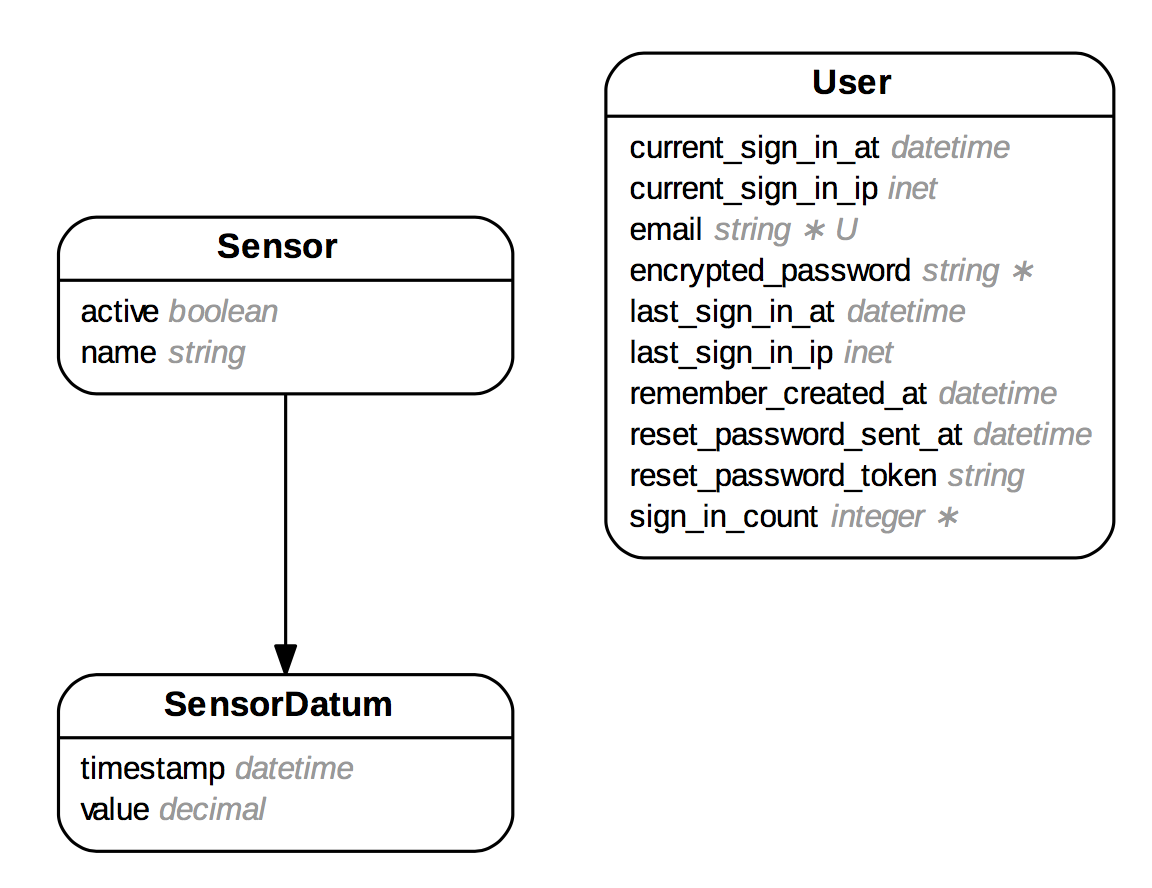
\includegraphics[width=\linewidth]{images/diagram_erd}
  \caption{Diagram ERD bazy danych.}
  \label{fig:diagram_erd}
\end{figure}
\newpage
\section{Ruby on Rails}
Framework \emph{Ruby on Rails} domyślnie korzysta z architektury \emph{MVC}. Aby nie łamać zasady \emph{Convention over Configuration}, zdecydowano się stworzyć aplikację zgodną z ideą frameworka, czyli w tej właśnie architekturze.

\subsection{Modele}
Aplikacja posiada 3 modele: \emph{User}, \emph{TemperatureSensor} oraz \emph{TemperatureSensorDatum}. Dodatkowo, korzystając z mechanizmu \emph{STI} (ang. \emph{Single Table Inheritation}), istnieją dwa modele abstrakcyjne \emph{Sensor} oraz \emph{SensorDatum}, które są bazą dla różnych typów sensorów oraz danych zbierane przez owe sensory. Na listingach \ref{lst:rails_sensor} oraz \ref{lst:rails_temp_sensor} przedstawiony jest przykład implementacji \emph{STI}, czyli abstrakcyjny model sensora oraz dziedziczący po nim model \emph{TemperatureSensor}.
\newpage

\begin{lstlisting}[caption={Abstrakcyjny model sensora w Ruby on Rails.},label={lst:rails_sensor},language=Ruby]
class Sensor < ApplicationRecord
end
\end{lstlisting}

\begin{lstlisting}[caption={Model sensora temperatury w Ruby on Rails.},label={lst:rails_temp_sensor},language=Ruby]
class TemperatureSensor < Sensor
  has_many :temperature_sensor_data
end
\end{lstlisting}

Łatwo zauważyć, że abstrakcyjny model jest praktycznie pusty. Jedyną ważną informacją jest dziedziczenie po klasie \emph{ApplicationRecord}, po której musi dziedziczyć każdy model. Natomiast w klasie \emph{TemperatureSensor} zdefiniowana jest relacja jeden do wielu z danymi sensora.

\subsection{Kontrolery}
\emph{Ruby on Rails} posiada mechanizm, który pozwala na wygenerowanie szablonu kontrolera. Zawarte są w nim implementacje podstawowych operacji typu \emph{CRUD}, czyli \textbf{C}reate - \textbf{R}ead - \textbf{U}pdate - \textbf{D}elete. Jako, że z założenia nie ma możliwości edycji przychodzących danych, pominięta została sekcja \emph{Update}. Kontroler odpowiedzialny za dane z sensorów temperatury przedstawiony jest na listingu \ref{lst:rails_temp_controller}.

\begin{lstlisting}[caption={TemperatureSensorDataController w Ruby on Rails.},label={lst:rails_temp_controller},language=Ruby]
class TemperatureSensorDataController < ApplicationController
  before_action :set_temperature_sensor_datum, only: :destroy

  # GET /temperature_sensor_data
  def index
    @temperature_sensor_data = TemperatureSensorDatum.all
  end

  # GET /temperature_sensor_data/new
  def new
    @temperature_sensor_datum = TemperatureSensorDatum.new
  end

  # POST /temperature_sensor_data
  def create
    @temperature_sensor_datum = TemperatureSensorDatum.new(temperature_sensor_datum_params)
    respond_to do |format|
      if @temperature_sensor_datum.save
        format.html { redirect_to temperature_sensor_data_url, notice: 'Temperature sensor datum was successfully created.' }
      else
        format.html { render :new }
        format.json { render json: @temperature_sensor_datum.errors, status: :unprocessable_entity }
      end
    end
  end

  # DELETE /temperature_sensor_data/1
  def destroy
    @temperature_sensor_datum.destroy
    respond_to do |format|
      format.html { redirect_to temperature_sensor_data_url, notice: 'Temperature sensor datum was successfully destroyed.' }
      format.json { head :no_content }
    end
  end

  private
    # Use callbacks to share common setup or constraints between actions.
    def set_temperature_sensor_datum
      @temperature_sensor_datum = TemperatureSensorDatum.find(params[:id])
    end

    # Never trust parameters from the scary internet, only allow the white list through.
    def temperature_sensor_datum_params
      params.require(:temperature_sensor_datum).permit(:value, :timestamp, :sensor_id)
    end
end
\end{lstlisting}

\subsection{Widoki}
Każda z akcji w kontrolerze powinna mieć swój odpowiednik w warstwie widoków. Framework \emph{Ruby on Rails} dostarcza mechanizm \emph{partial'i}, który pozwala podział widoków na kilka plików w celu umożliwienia korzystania z jednego fragmentu w kilku miejscach. Przykład takiego rozwiązania można pokazać jako podstronę dodawania nowej próbki danych z sensora (listing \ref{lst:rails_sensor_data_view}), gdzie sam formularz jest reużywalnym fragmentem - \emph{partial'em} (listing \ref{lst:rails_sensor_form_partial}).

\begin{lstlisting}[caption={Widok, na którym można dodać nowe próbki dla sensora temperatury.},label={lst:rails_sensor_data_view},language=Ruby]
<h1>New Temperature Sensor Datum</h1>

<%= render 'form', temperature_sensor_datum: @temperature_sensor_datum %>

<%= link_to 'Back', temperature_sensor_data_path %>
\end{lstlisting}

\begin{lstlisting}[caption={Fragment, na którym jest formularz.},label={lst:rails_sensor_form_partial},language=Ruby]
<%= form_for(temperature_sensor_datum) do |f| %>
  <% if temperature_sensor_datum.errors.any? %>
    <div id="error_explanation"\>
      <h2><%= pluralize(temperature_sensor_datum.errors.count, "error") %> prohibited this temperature_sensor_datum from being saved:</h2>

      <ul>
      <% temperature_sensor_datum.errors.full_messages.each do |message| %>
        <li><%= message %></li>
      <% end %>
      </ul>
    </div>
  <% end %>

  <div class="field"\>
    <%= f.label :value %>
    <%= f.number_field :value, { step: 0.1 } %>
  </div\>

  <div class="field"\>
    <%= f.label :timestamp %>
    <%= f.datetime_local_field :timestamp %>
  </div>

  <div class="field"\>
    <%= f.label :sensor_id %>
    <%= f.collection_select(:sensor_id, TemperatureSensor.where(active: true), :id, :name) %>
  </div>

  <div class="actions"\>
    <%= f.submit %>
  </div>
<% end %>
\end{lstlisting}

\subsection{Przetwarzanie w tle - ActiveJob}
Framework \emph{Ruby on Rails} posiada wbudowany mechanizm, który jest abstrakcją umożliwiającą przetwarzanie danych w tle - \emph{ActiveJob}. Biblioteka ta posiada szereg adapterów do najbardziej popularnych mechanizmów zajmujących się owym przetwarzaniem. Dzięki temu możliwa jest ewentualna zmiana samego narzędzia, przy zachowaniu kodu. W aplikacji wykorzystane zostało narzędzie \emph{Sidekiq}.

Sam proces przetwarzania składa się z trzech części - widoku z formularzem, przy pomocy którego użytkowniok może wysłać plik csv na serwer, akcji w kontrolerze, która odbiera plik i przekazuje go do ostatniego etapu, czyli przetwarzania w tle. Na listingu \ref{lst:rails_active_job} przedstawiony został ostatni etap tego procesu.

\begin{lstlisting}[caption={},label={lst:rails_active_job},language=Ruby]
require "csv"
class UserImportJob < ApplicationJob
  queue_as :default

  def perform(file)
    CSV.foreach(file.path) do |row|
      User.create!(row.to_h)
    end
  end
end
\end{lstlisting}

\section{Phoenix}
\emph{Phoenix}, podobnie jak \emph{Ruby on Rails}, jest frameworkiem korzystającym z architektury \emph{Model-View-Controller}.

\subsection{Modele}
Jako, że \emph{Phoenix} nie posiada wbudowanego mechanizmu \emph{STI}, każdy model korzysta z osobnej tabeli w bazie danych. Oznacza to brak abstrakcyjnych modeli i ilość tabel w bazie danych równą ilości używanych modeli. Framework ten w modelu, poza relacjami z innymi modelami, przechowuje schemat danych w tabeli, z której korzysta dany model.

\begin{lstlisting}[caption={Model sensora temperatury we frameworku Phoenix.},label={lst:phoenix_temp_sensor_model}]
defmodule App.TemperatureSensor do
  use App.Web, :model

  schema "temperature_sensors" do
    field :name, :string
    field :active, :boolean, default: false

    timestamps()
  end

  def changeset(struct, params \\ %{}) do
    struct
    |> cast(params, [:name, :active])
    |> validate_required([:name, :active])
  end
end
\end{lstlisting}


\subsection{Kontrolery}
\emph{Phoenix} posiada mechanizm generowania \emph{scaffoldów}, które bardzo przyspieszają tworzenie aplikacji i generują sporą część kodu kontrolera, dzięki czemu można tworzyć proste aplikacje z minimalną znajomością języka programowania \emph{Elixir}. \emph{Scaffold} domyślnie generuje akcje kontrolera w konwencji \emph{CRUD}, lecz aby aplikacja była zgodna z wcześniejszymi założeniami, usunięta została część odpowiedzialna za edycję danych. Kontroler po tych zmianach przedstawiony jest na listingu \ref{lst:phoenix_controller}.

\begin{lstlisting}[caption={Kontroler danych z sensorów temperatur we frameworku Phoenix},label={lst:phoenix_controller}]
defmodule App.TemperatureSensorDatumController do
  use App.Web, :controller
  require IEx

  alias App.TemperatureSensorDatum
  alias App.TemperatureSensor

  def index(conn, _params) do
    temperature_sensor_data = Repo.all(TemperatureSensorDatum)
    render(conn, "index.html", temperature_sensor_data: temperature_sensor_data)
  end

  def new(conn, _params) do
    changeset = TemperatureSensorDatum.changeset(%TemperatureSensorDatum{})
    query = from(s in TemperatureSensor, select: {s.name, s.id})
    sensors = Repo.all(query)
    render(conn, "new.html", changeset: changeset, sensors: sensors)
  end

  def create(conn, %{"temperature_sensor_datum" => temperature_sensor_datum_params}) do
    temperature_sensor_datum_params =
      if temperature_sensor_datum_params["utc_timestamp"] do
        {:ok, timestamp} = DateTime.from_unix!(temperature_sensor_datum_params["utc_timestamp"])
        Map.put(temperature_sensor_datum_params, "utc_timestamp", timestamp)
      else
        temperature_sensor_datum_params
      end
    changeset = TemperatureSensorDatum.changeset(%TemperatureSensorDatum{}, temperature_sensor_datum_params)

    case Repo.insert(changeset) do
      {:ok, _temperature_sensor_datum} ->
        conn
        |> put_flash(:info, "Temperature sensor datum created successfully.")
        |> redirect(to: temperature_sensor_datum_path(conn, :index))
      {:error, changeset} ->
        query = from(s in TemperatureSensor, select: {s.name, s.id})
        sensors = Repo.all(query)
        render(conn, "new.html", changeset: changeset, sensors: sensors)
    end
  end

  def show(conn, %{"id" => id}) do
    temperature_sensor_datum = Repo.get!(TemperatureSensorDatum, id)
    render(conn, "show.html", temperature_sensor_datum: temperature_sensor_datum)
  end

  def delete(conn, %{"id" => id}) do
    temperature_sensor_datum = Repo.get!(TemperatureSensorDatum, id)

    # Here we use delete! (with a bang) because we expect
    # it to always work (and if it does not, it will raise).
    Repo.delete!(temperature_sensor_datum)

    conn
    |> put_flash(:info, "Temperature sensor datum deleted successfully.")
    |> redirect(to: temperature_sensor_datum_path(conn, :index))
  end
end
\end{lstlisting}

\subsection{Widoki}
W kwestii warstwy prezentacji widoczna jest inspiracja frameworkiem \emph{Ruby on Rails}. \emph{Phoenix} również posiada mechanizm fragmentów i działa on na takiej samej zasadzie, jak w oryginale.
\newpage

\begin{lstlisting}[caption={Widok, na którym można dodać dane dla sensora w  Phoenix'ie.},label={lst:phoenix_new_data_view},language=HTML]
<h2>New temperature sensor datum</h2>

<%= render "form.html", changeset: @changeset,
                        action: temperature_sensor_datum_path(@conn, :create),
                        sensors: @sensors %>

<%= link "Back", to: temperature_sensor_datum_path(@conn, :index) %>
\end{lstlisting}

\begin{lstlisting}[caption={Fragment, na którym jest formularz we frameworku Phoenix.},label={lst:phoenix_sensor_form_partial},language=HTML]
<%= form_for @changeset, @action, fn f -> %>
  <%= if @changeset.action do %>
    <div class="alert alert-danger"\>
      <p>Oops, something went wrong! Please check the errors below.</p>
    </div>
  <% end %>

  <div class="form-group"\>
    <%= label f, :value, class: "control-label" %>
    <%= number_input f, :value, step: "any", class: "form-control" %>
    <%= error_tag f, :value %>
  </div>

  <div class="form-group"\>
    <%= label f, :timestamp, class: "control-label" %>
    <%= datetime_select f,  :timestamp, class: "form-control" %>
    <%= error_tag f, :timestamp %>
  </div>

  <div class="form-group"\>
    <%= label f, :sensor_id, class: "control-label" %>
    <%= select(f, :sensor_id, @sensors) %>
  </div>

  <div class="form-group"\>
    <%= submit "Submit", class: "btn btn-primary" %>
  </div>
<% end %>
\end{lstlisting}

\subsection{Przetwarzanie danych w tle}
\emph{Phoenix} nie posiada wbudowanej biblioteki, która nakłada abstrakcję i unifikuje dostęp do mechanizmów odpowiedzialnych za przetwarzanie w tle. Nie oznacza to jednak, że realizacja przetwarzania danych w tle jest niemożliwa. Z pomocą przychodzi biblioteka \emph{Exq}. Sugeruje ona rozszerzenie istniejącej struktury o \emph{Workery}. Zaimplementowany \emph{worker} został przedstawiony na listingu \ref{lst:phoenix_worker}.

\begin{lstlisting}[caption={Worker umożliwiający import użytkowników z pliku csv we frameworku Phoenix.},label={lst:phoenix_worker}]
defmodule App.ImportUsersWorker do

  def perform(file) do
    File.stream!(file.path)
      |> CSV.decode(separator: ?;) |>
        Enum.each(fn row ->
          res = %{
            email: Enum.at(row, 0),
            password: Enum.at(row, 1),
            password_confirmation: Enum.at(row, 1)
          }
          User.changeset(%User{}, res)
          |> Repo.insert
        end)
  end
end
\end{lstlisting}

Aby dodać zadanie do kolejki, z poziomu kontrolera należy wywołać metodę przedstawioną na listingu \ref{lst:phoenix_worker_ctrl}

\begin{lstlisting}[caption={Dodanie zadania do kolejki przetwarzania w tle we frameworku Phoenix.},label={lst:phoenix_worker_ctrl}]
def import(conn, params) do
  {:ok, jid} = Exq.enqueue(Exq, "default", "ImportUsersWorker", [params["import"]["csv"]])
  text conn, "Task scheduled"
end
\end{lstlisting}

\section{Express}
\subsection{Modele}

\subsection{Kontrolery}

\subsection{Widoki}


\chapter{Analiza wydajnościowa}

\section{Metody mierzenia wydajności aplikacji internetowych}
Głównym problemem aplikacji internetowych jest sytuacja, gdy w jednym momencie próbuje z niej skorzystać duża ilość użytkowników. Błędy aplikacji objawiają się wtedy poprzez długi czas przetwarzania, błąd przetwarzania bądź też odrzucenie zapytania HTTP. Oczywiście takie zachowanie jest bardzo niepożądane, dlatego też nowoczesne frameworki starają się minimalizować możliwość wystąpienia takich sytuacji.

Z tego też powodu aplikacjie poddawane są testom obciążeniowym. Tego typu testy opierają się na symulacji dużej liczby użytkowników próbujących skorzystać z aplikacji i analizie odpowiedzi z aplikacji. Na podstawie testów można uzyskać dane m.in. na temat:
\begin{itemize}
  \item procentowej ilości błędów,
  \item wartości minimalnej, maksymalnej, średniej i medianie czasu odpowiedzi,
  \item rozmiaru odpowiedzi z serwera,
  \item średniej ilości przetworzonych zapytań w jednostce czasu.
\end{itemize}


\section{Wyniki badań}
Badania zostały przeprowadzone na serwerze \emph{VPS} firmy \emph{DigitalOcean}. Posiada ona następujące parametry:
\begin{itemize}
  \item procesor: dwurdzeniowy Intel(R) Xeon(R) CPU E5-2650L v3 @ 1.80GHz,
  \item pamięć RAM: 2GB,
  \item dysk: 40GB SSD,
  \item system operacyjny: Ubuntu 16.04.2 LTS (Xenial Xerus)
\end{itemize}

Zgodnie z zaprojektowanym środowiskiem eksperymentalnym, testy wydajnościowe zostały przeprowadzone z wykorzystaniem narzędzia \emph{Locust}. Wyniki badań są uśrednionymi wartościami z 10 przebiegów testowych.

\subsection{Czas odpowiedzi z serwera}
W kategorii czasu odpowiedzi z serwera mierzone były następujące wartości:
\begin{itemize}
  \item mediana czasu odpowiedzi,
  \item średnia czas odpowiedzi,
  \item minimalny czas odpowiedzi,
  \item maksymalny czas odpowiedzi.
\end{itemize}

Wyniki dla poszczególnych frameworków przedstawione są w tabeli \ref{tab:czas_odp}.

\begin{table}[h]
\centering
\caption{Wyniki badań czasu odpowiedzi.\\Źródło: opracowanie własne.}
\label{tab:czas_odp}
\begin{tabular}{|l|l|l|l|l|}
\hline
              & \textbf{Mediana {[}ms{]}} & \textbf{Średnia {[}ms{]}} & \textbf{Min {[}ms{]}} & \textbf{Max {[}ms{]}} \\ \hline
\textbf{Ruby on Rails} & 160000           & 184060           & 114          & 544870       \\ \hline
\textbf{Phoenix}       & 23000            & 31873            & 623          & 169825       \\ \hline
\textbf{Express}       & 32000            & 33193            & 1514         & 112874       \\ \hline
\end{tabular}
\end{table}

Już podczas analizy wyników w formie tabelarycznej można zauważyć dużo większe wartości przy frameworku \emph{Ruby on Rails}. Różnice te są dużo bardziej widoczne na zestawieniu pokazanym w formie wykresu słupkowego przedstawionego na rysunku \ref{fig:response_times}.
\newpage
\begin{figure}[h]
  \centering
  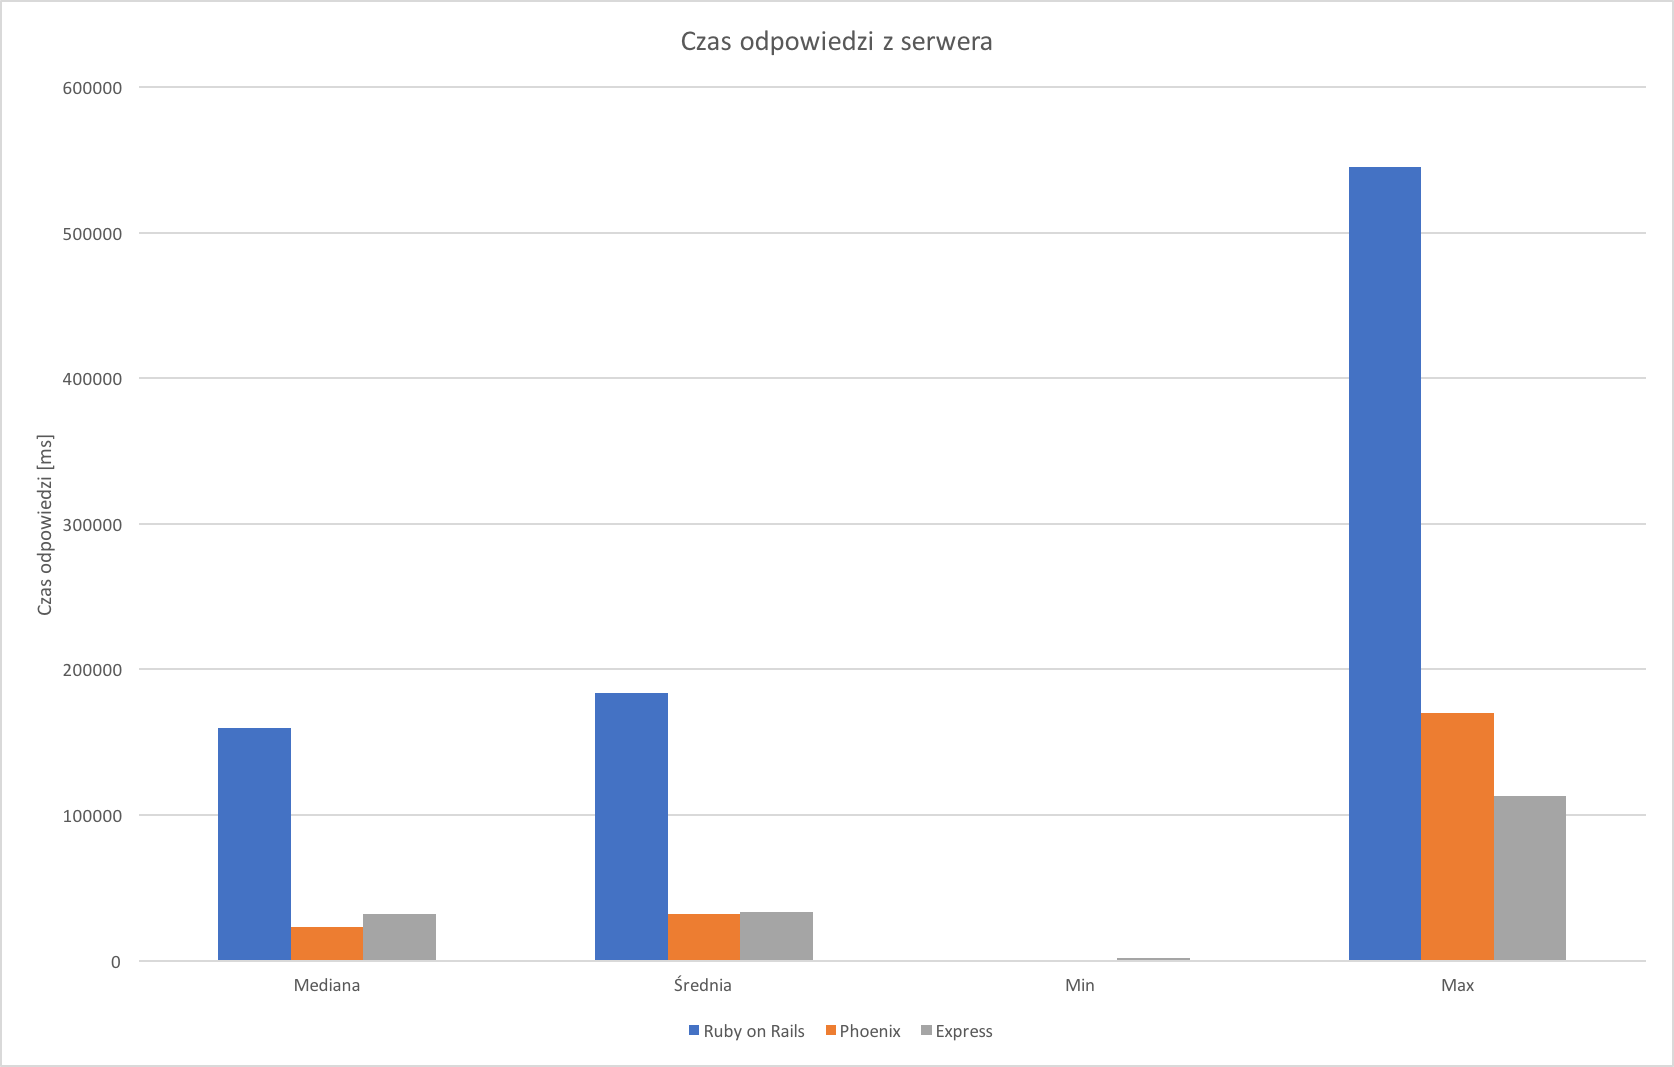
\includegraphics[width=\linewidth]{images/response_times}
  \caption{Porównanie czasów odpowiedzi z serwera.\\Źródło: opracowanie własne.}
  \label{fig:response_times}
\end{figure}

Zgodnie z przewidywaniami, \emph{Ruby on Rails} jest najwolniejszym frameworkiem, jeśli chodzi o czas odpowiedzi z serwera. Średni czas odpowiedzi jest ok. 5,5 razy większy niż w przypadku pozostałych frameworków. Spowodowane jest to faktem, iż język \emph{Ruby} nie należy do najszybszych języków programowania. Jego celem miało być dostarczenie przyjemności z programowania, co niestety odbiło się negatywnie na wydajności.

Najszybszym frameworkiem okazał się, zgodnie z oczekiwaniami, \emph{Phoenix}. Twórcom udało się zrealizować założenie dotyczące wydajności tego frameworka. Wpływ ma na to oczywiście wspomniany wcześniej język \emph{Elixir}. Co ciekawe, wydajność ta została osiągnięta z zachowaniem przyjemności z tworzenia aplikacji, co potwierdza duży potencjał tego frameworka.

Zaskoczeniem jest wydajność frameworka \emph{Express}. W zestawieniu jest on minimalnie wolniejszy od \emph{Phoenix'a}, co można określić jako bardzo dobry wynik. Wpływ na to ma minimalizm tego narzędzia. \emph{Express} z racji na swoją ,,ubogość'' domyślnych bibliotek jest bardzo małym frameworkiem. W połączeniu z szybką platformą \emph{Node.js}, która odpowiedzialna jest za serwowanie aplikacji, otrzymane zostały bardzo dobre wyniki czasu odpowiedzi.

\subsection{Ilość obsłużonych zapytań na sekundę}
Poza czasem odpowiedzi bardzo ważnym parametrem jest ilość obsłużonych zapytań na sekundę. Analiza tego parametru pozwala określić ilu użytkowników może jednocześnie korzystać z systemu bez problemów z wydajnością. Efektem owej analizy może być decyzja o zwiększeniu mocy obliczeniowej maszyny, która obsługuje aplikację bądź też zastosowanie \emph{load balancing'u}. Wyniki przeprowadzonych badań zostały przedstawione w tabeli \ref{tab:rps} oraz na wykresie \ref{fig:rps}.

\begin{table}[h]
\centering
\caption{Wyniki badań ilości zapytań na sekundę.}
\label{tab:rps}
\begin{tabular}{|l|l|}
\hline
                       & \textbf{RPS} \\ \hline
\textbf{Ruby on Rails} & 4,74         \\ \hline
\textbf{Phoenix}       & 9,86         \\ \hline
\textbf{Express}       & 22,09        \\ \hline
\end{tabular}
\end{table}

\begin{figure}[h]
  \centering
  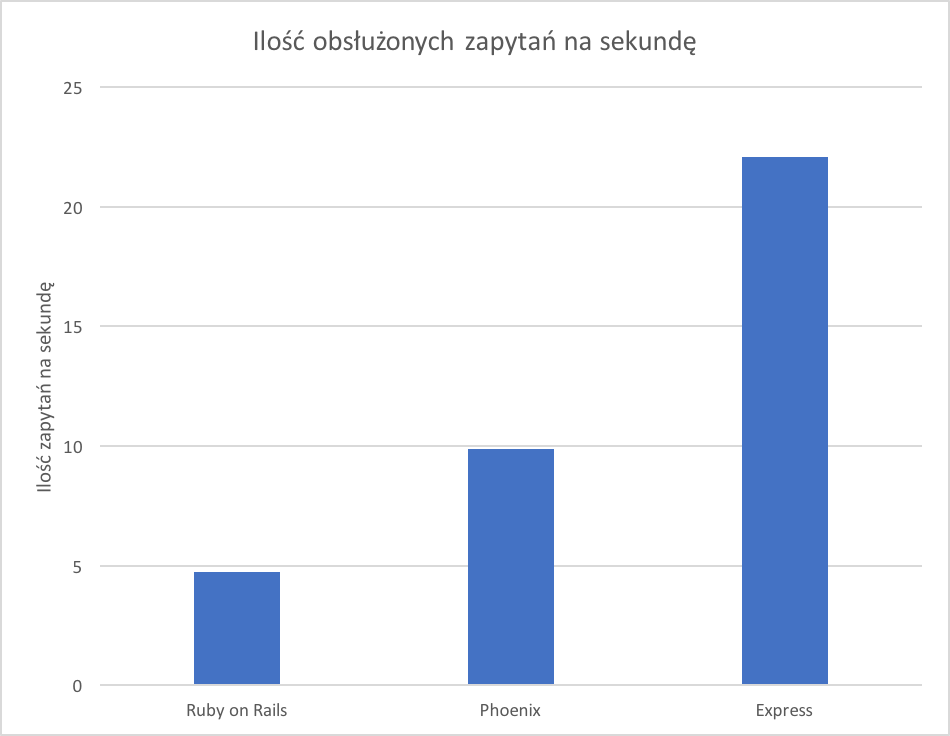
\includegraphics[width=0.7\linewidth]{images/rps}
  \caption{Porównanie ilości obsłużonych zapytań na sekundę.\\Źródło: opracowanie własne.}
  \label{fig:rps}
\end{figure}

Wyniki tych badań są nieco zaskakujące. Najwięcej zapytań, z ponad dwukrotnie lepszym wynikiem niż drugi w zestawieniu \emph{Phoenix}, obsłużył framework \emph{Express}. Przyczyn takiego wyniku ponownie można doszukiwać się w platformie \emph{Node.js}, na której oparty jest ten framework. Jest ona bardzo stabilna i stanowi podstawę dla wielu frameworków, w tym frontendowych, co doprowadziło do optymalizacji wydajności.

Drugi pod względem ilości przetworzonych zapytań na sekundę jest framework \emph{Phoenix}. Przed przeprowadzeniem testów, framework ten był faworytem w osiągnięciu najlepszego wyniku ze względu na język \emph{Elixir}, który pochodzi od \emph{Erlang'a}, a więc jest językiem posiadającym mechanizm \emph{lekkich wątków} (mechanizm podobny do \emph{zielonych wątków}). Testy jednak jednoznacznie pokazały, iż ilość obsłużonych zapytań w czasie sekundy nie jest wyjątkowo duża.

Frameworkiem, który zdołał obsłużyć najmniej zapytań w ciągu sekundy, został \emph{Ruby on Rails}. Także w tym przypadku taki wynik był zgodny z przewidywaniami. \emph{Ruby on Rails} jest 2 razy wolniejszy od \emph{Phoenix'a} i aż 4 razy wolniejszy od \emph{Express'a}. Pokazuje to, że framework ten, zgodnie z jego założeniami, powinien być stosowany głównie w celu prototypowania aplikacji.

\subsection{Poprawność odpowiedzi z serwera}
Poza szybkością działania aplikacji, bardzo ważnym elementem aplikacji internetowych jest ich niezawodność. Nawet jeśli framework jest wydajny, to traci on na wartości, jeśli nie jest niezawodny. W tym celu przeprowadzone zostały badania niezawodności. Ich wynikiem jest procentowa ilość błędów w odniesieniu do ilości zapytań. Wyniki w formie tabelarycznej oraz wykresu są przedstawione poniżej.

\begin{table}[h]
\centering
\caption{Wyniki ilości błędów zapytań w odniesieniu do ilości zapytań.}
\label{tab:poprawnosc}
\begin{tabular}{|l|l|}
\hline
                       & \textbf{Ilość błędów [\%]} \\ \hline
\textbf{Ruby on Rails} & 0,41         \\ \hline
\textbf{Phoenix}       & 9,01         \\ \hline
\textbf{Express}       & 0,00        \\ \hline
\end{tabular}
\end{table}

\newpage

\begin{figure}[h]
  \centering
  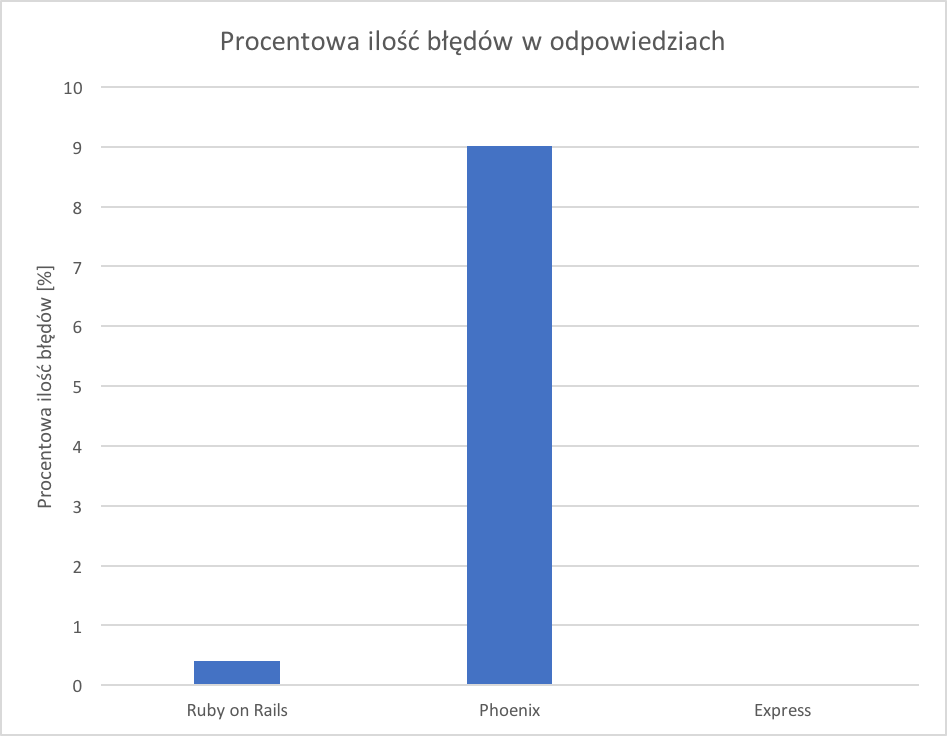
\includegraphics[width=0.7\linewidth]{images/errors}
  \caption{Zestawienie ilości błędnych odpowiedzi z serwerów.\\Źródło: opracowanie własne.}
  \label{fig:rps}
\end{figure}

Wyniki otrzymane na podstawie badań odpowiadają przewidywanym wynikom. \emph{Ruby on Rails} osiągnąl ilość błędów na poziomie $0,41\%$. Jest to wynik bardzo dobry, biorąc pod uwagę obciążenie, któremu została poddana aplikacja. I stanowczo jest to wynik mieszczący się w dopuszczalnych granicach błędów, które nie wpływają negatywnie na odczucia użytkownika.

Niewielką niespodzianką jest wynik frameworka \emph{Phoenix}. $9\%$ błednych odpowiedzi jest dużą wartością. Wynik ten można tłumaczyć jedynie młodym wiekiem tego rozwiązania, ponieważ \emph{Elixir} z założenia stawia na niezawodność. Stanowczo jest to element, który powinien zostać dopracowany w kolejnych wersjach frameworka.

Wręcz idealny wynik osiągnął \emph{Express}. W trakcie badań jego ilość błędów utrzymywała się na poziomie $0\%$, co oznacza pełną niezawodność. Przyczyną takiego wyniku jest niewątpliwie niewielki rozmiar frameworka. Oczywistym jest, że im mniej elementów może wygenerować błąd, tym większa niezawodność systemu.

\section{Wnioski z badań}
Na podstawie badań można wysnuć kilka wniosków. Po pierwsze - założenia frameworka nie zawsze pokrywają się z rzeczywistością. Przykładowo, \emph{Phoenix} reklamowany jest jako framework stawiający na szybkość działania, skalowalność i niezawodność. W przypadku pierwszych dwóch własności cel został osiągnięty (chociaż np. w porównaniu do \emph{Express'a} nie jest to wynik dużo lepszy). Problemem jest niestety niezawodność. Nawet najszybszy framework nie będzie wykorzystywany w momencie, kiedy nie jest niezawodny.

Po drugie, minimalizm, szczególnie pod względem wydajności, jest korzystny. Oczywiście taką aplikację trudniej się pisze oraz jest ryzyko, że mimo wszystko rozrośnie się do dużych rozmiarów. Mimo wszystko jeśli ktoś poszukuje wydajności, powinien skorzystać z \emph{Express'a} lub podobnych do niego frameworków.


\chapter{Podsumowanie}


\renewcommand\bibname{Literatura}
\begin{thebibliography}{inteligencja}
	\addcontentsline{toc}{chapter}{Literatura}

  \bibitem{historia}
  \emph{Historia Internetu}, dostęp pod adresem: \url{https://pl.wikipedia.org/wiki/Historia_Internetu}, aktualne na dzień 1.04.2017r.

  \bibitem{framework}
  \emph{Software framework}, dostęp pod adresem: \url{https://en.wikipedia.org/wiki/Software_framework}, aktualne na dzień 1.04.2017r.

	\bibitem{rails_guide}
	\emph{Ruby on Rails Guides}, dostęp pod adresem: \url{http://guides.rubyonrails.org/},\\ aktualne na dzień 14.06.2017r.

  \bibitem{rails_doctrine}
  \emph{Ruby on Rails Doctrine}, dostęp pod adresem: \url{http://rubyonrails.org/doctrine/}, aktualne na dzień 1.05.2017r.

  \bibitem{phoenix_doctrine}
  McCord R., Tate B., Valim J., \emph{Programming Phoenix}, The Pragmatic Programmers LLC, 2016

  \bibitem{phoenix_docs}
  \emph{Phoenix Guides}, dostęp pod adresem: \url{http://www.phoenixframework.org/docs/resources}, aktualne na dzień 6.05.2017r.

	\bibitem{cleancode}
	Martin, R. \emph{Czysty kod. Podręcznik dobrego programisty}, Gliwice, Wydawnictwo Helion 2010

  \bibitem{benchmarking_tools}
  Diwan, A. \emph{Tools for Testing Website Performance}, dostęp pod adresem: \url{https://www.sitepoint.com/tools-testing-website-performance/}, \\ aktualne na dzień 18.03.2017r.

  \bibitem{dry}
  \emph{Don't Repeat Yourself}, dostęp pod adresem: \url{http://deviq.com/don-t-repeat-yourself/}, aktualne na dzień 3.05.2017r.

  \bibitem{docker_what_container}
  \emph{What is a Container}, dostęp pod adresem: \url{https://www.docker.com/what-container}, aktualne na dzień 27.05.2017r.

  \bibitem{docker_prez}
  \emph{Docker. Kontener aplikacyjny nie tylko dla programistów}, dostęp pod adresem: \url{https://dsg.cs.put.poznan.pl/wiki/_media/workshop/docker-skisr.pdf}, aktualne na dzień 27.05.2017r.

  \bibitem{wiki_crud}
  \emph{CRUD}, dostęp pod adresem: \url{https://pl.wikipedia.org/wiki/CRUD}, aktualne na dzień 27.05.2017r.

  \bibitem{elixir}
  \emph{Elixir Language}, dostęp pod adresem: \url{https://elixir-lang.org/}, aktualne na dzień 16.05.2017r.

  \bibitem{elixir_medium}
  Mazaika, K. \emph{Why I'm betting on Elixir}, dostęp pod adresem: \url{https://medium.com/@kenmazaika/why-im-betting-on-elixir-7c8f847b58}, aktualne na dzień 28.05.2017r.

  \bibitem{express}
  \emph{Express Guides}, dostęp pod adresem: \url{https://expressjs.com/}, aktualne na dzień 10.06.2017r.

  \bibitem{express_pro}
  % http://www.apress.com/gp/book/9781484200384
  Mardanm A. \emph{Pro Express.js}, Apress, 2014

  \bibitem{npm_site}
  \emph{npm Homepage}, dostęp pod adresem: \url{https://www.npmjs.com/}, aktualne na dzień 10.06.2017r.

\end{thebibliography}
\end{document}
